\chapter{Backward compatibility} \label{Chp:backward}

\dfastmi may be run in \keyw{cli} mode for backward compatible with WAQMORF: in this (legacy) mode the configuration for the analysis is obtained by asking the user questions via a command line interface which support simulation results from WAQUA only.
The input and output as well as the description of the conceptual framework of that version is described in this appendix.

\dfastmi can also be run in backward compatible \keyw{batch} mode by specifying version 1 files for the rivers configuration and analysis configuration.

\section{Running in interactive command line mode}

The cli mode runs an interactive command line analysis using WAQUA results; this run mode does not support \dflowfm files.
The program should be started with the run mode set to \keyw{cli} on the command line as follows

\begin{Verbatim}
> dfastmi --mode cli
\end{Verbatim}

You may choose to run the program in either Dutch \keyw{-{}-language NL} (like the original WAQMORF) or English \keyw{-{}-language UK}; the latter is the default.
Please note that the language not only affects the text in the report, but also the names of the output files as indicated in the opening section of this chapter.
You may also choose to select the \keyw{-{}-reduced\_output} option for smaller SIMONA BOX file output.
When the program is started in this way, the program will ask you questions on the command line.
An example of the dialog is given in \autoref{Sec:cli_dialog}.
Because the \dfmi binary distributed suppresses the DOS box, this backward compatibility option is currently not accessible interactively.
Although this run mode is designed as an interactive dialog, you may use this mode also as a batch mode by redirecting standard input to read from file as follows

\begin{Verbatim}
> dfastmi --mode cli < myfile.in
\end{Verbatim}

In this case each line in the file \file{myfile.in} should contain the appropriate answer to the question.
This run mode is included for backward compatibility and comparison with its predecessor WAQMORF.
It should not be used for new studies based on \dflowfm results.

\section{Output files}

The \emph{cli mode} produces the following four output files:

\begin{itemize}
\item Text file with summary report of the analysis \\
English: \keyw{report.txt} \\
Dutch: \keyw{verslag.run}
\item Average yearly change in SIMONA BOX file format (when the analysis runs using WAQUA input) \\
English: \keyw{yearavg\_dzb.out} \\
Dutch: \keyw{jaargem.out}
\item Maximum change in SIMONA BOX file format (when the analysis runs using WAQUA input) \\
English: \keyw{max\_dzb.out} \\
Dutch: \keyw{maxmorf.out}
\item Minimum change in SIMONA BOX file format (when the analysis runs using WAQUA input) \\
English: \keyw{min\_dzb.out} \\
Dutch: \keyw{minmorf.out}
\end{itemize}

\section{Conceptual framework}

This section describes the conceptual framework of the method used by \dfastmi version 2, and by version 3 in backward compatibility mode, and the derivation of the river parameters used for the Dutch rivers.

\subsection{Characteristics of bed level changes due to river interventions}

A river intervention, i.e.~a local river adjustment (typically a flow capacity enlarging adjustment) outside the main channel, may result in changes in the flow pattern within the main channel.
The bed levels within the main channel will react to such changes depending on the

\hspace{1cm}\emph{magnitude, duration and length scale of these flow pattern changes in the main channel.}

Hence, the core focus of the rule-of-thumb is to determine and characterize the changes in the flow pattern within the main channel.
Here, we define the main channel as the part of the river between the groyne heads.

At the upstream end of the floodplain adjustment part of the main channel discharge will leave the main channel, which will flow through the enlarged floodplain, secondary channel or bank area, and return to the main channel at the downstream end of the project area.
The resulting changes in the main channel flow pattern cause sedimentation in the main channel at the upstream "offtake" of the new outflow and erosion at the downstream "confluence" when the flow enters the main channel again.
Because the river discharge varies, the pattern will also vary during the year
As a result a part of the main channel bed level adjustment is stationary and a part of the adjustment is transitional and it will migrate downstream.
A reduction in the water depth may thus not only be observed locally where the flow diverges into the flood plain, but also downstream thereof.

The bed level change due to river enlargement can largely be characterized as follows

\begin{itemize}
\item The magnitude of the bed level change varies over the seasons; the maximum change is observed at the end of the flood season and the adjustment reaches a minimum at the end of the low flow period.

\item Local evaluation of the bed level changes is insufficient because of partial downstream migration of the bed level changes.

\item The maximum impact is observed on that side of the river which is closest to the adjustment.
\end{itemize}

Because part of the bed level changes migrate downstream, the morphological impact on projects located downstream may be increased.
After all, the maximum bed level change of one single river enlarging intervention is reached at the end of the flood period and it's the result of that flood period.
However, when a series of interventions along the river are combined (for instance, lowering of the groynes along a reach) the downstream bed level changes may be increased by accumulation of downstream migrating bed waves, such that the accumulated bed level change may be significantly larger.
In other words, river interventions extending over longer reaches may result in a larger morphodynamic response than comparable but more isolated interventions.

The aforementioned observations result in the following premises.
The rule-of-thumb described in the following sections

\begin{itemize}
\item will only be valid for the estimation of the impact of local interventions with a length of at most one flood plain,

\item should take into account seasonal variations, and

\item needs to be estimate the spatial pattern of the bed level change.
\end{itemize}


\subsection{Characterization of the changes in the main channel flow pattern}

When an intervention in the floodplains does not include something like a permanently active secondary channel, the flow pattern in the main channel will only be affected during flood conditions.
If on the other hand, such a secondary channel (or other intervention active under medium to low flow conditions such as groyne adjustments) is included in the design then the flow pattern will also be influenced during transitional or even low flow conditions.
It's therefore critical to determine the effect of the intervention on the main channel flow pattern at different discharge levels.

Secondary channels may have a major impact on the morphodynamics of the main channel.
The magnitude of the discharge through the secondary channel varies as function of the river discharge.
Because the hydraulic conditions of the secondary channel can change over time (e.g.~due to vegetation, siltation, or erosion) the discharge through a secondary channel is typically controlled by some hydraulic structure.
The typical characteristics of a weir (overlaat, drempel) and orifice (onderlaat, duiker) are shown in \autoref{App.Fig1}.

\begin{figure}
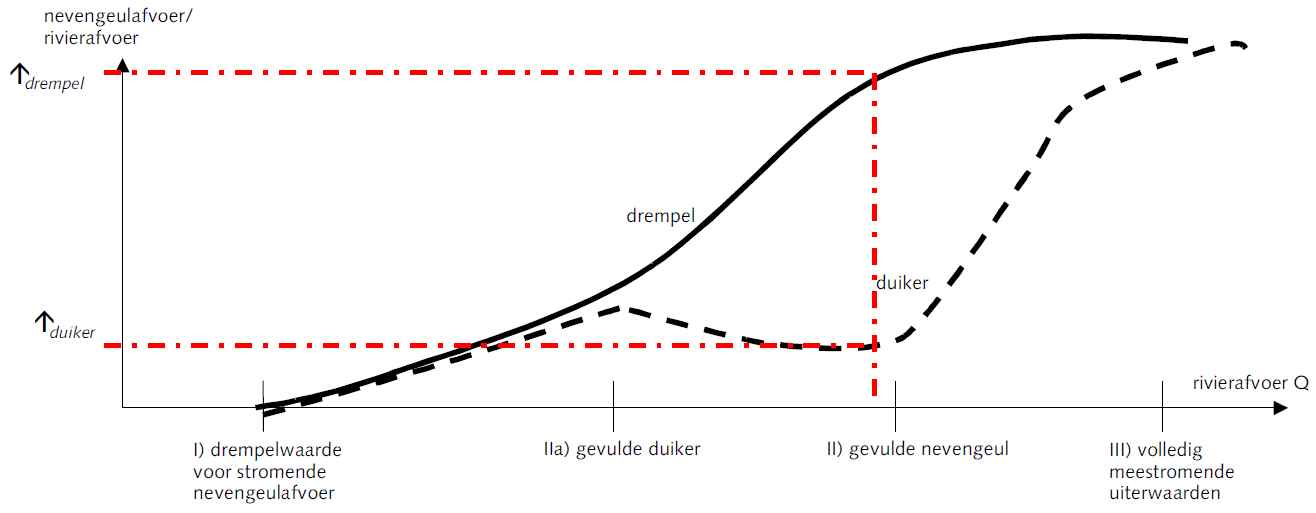
\includegraphics[width=\columnwidth]{figures/Fig1.png}
\caption{Schematic of the controlled discharge through a secondary channel.}
\label{App.Fig1}
\end{figure}

The discharge through a secondary channel is characterized by a number of special conditions as illustrated by \autoref{App.Fig1}:

\begin{enumerate}
\item the beginning of flow through the secondary channel
\item the bankfull secondary channel
\item the fully developed flow in the secondary channel and surrounding floodplain.
\end{enumerate}

When the discharge through the secondary channel is controlled by an orifice, the fully flooded condition may add an additional characteristic discharge.

In order to characterize the flow patterns during flood it's necessary to distinguish the condition in which the flood plains just start to carry flows, and the condition of fully developed flow in the flood plains.
Based on results of 1D simulations shown in \autoref{App.Fig2a} it has been concluded that for the Rhine branches a discharge of 6000 m\textsuperscript{3}/s at Lobith can be used as the boundary between those two conditions.
The flow through the bank zone (\autoref{App.Fig2b}) is also largely developed for discharges at Lobith larger than
6000 m\textsuperscript{3}/s.

\begin{figure}
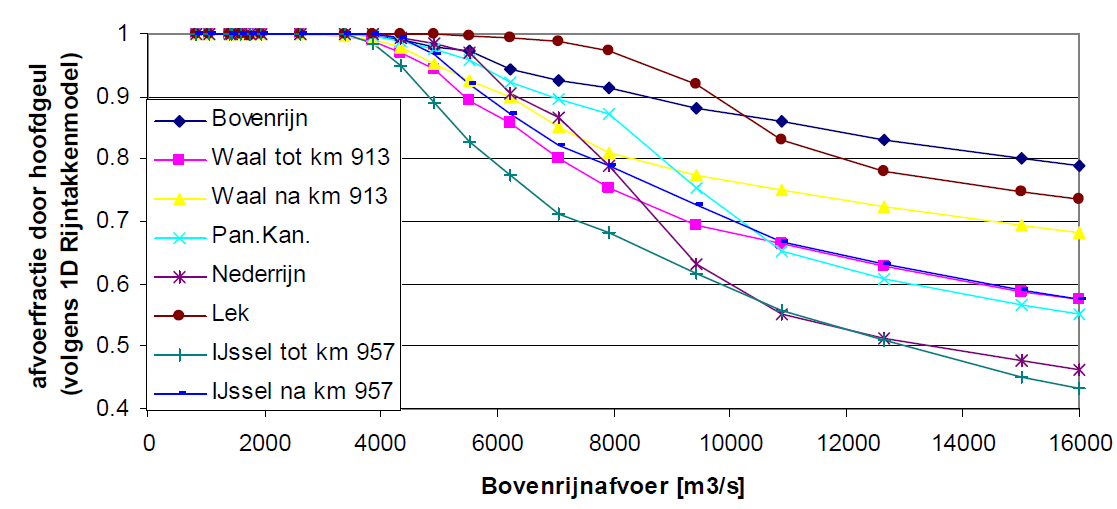
\includegraphics[width=\columnwidth]{figures/Fig2a.png}
\caption{Reach-averaged discharge fraction through the main channel (based on 1D model of the Rhine branches).}
\label{App.Fig2a}
\end{figure}

\begin{figure}
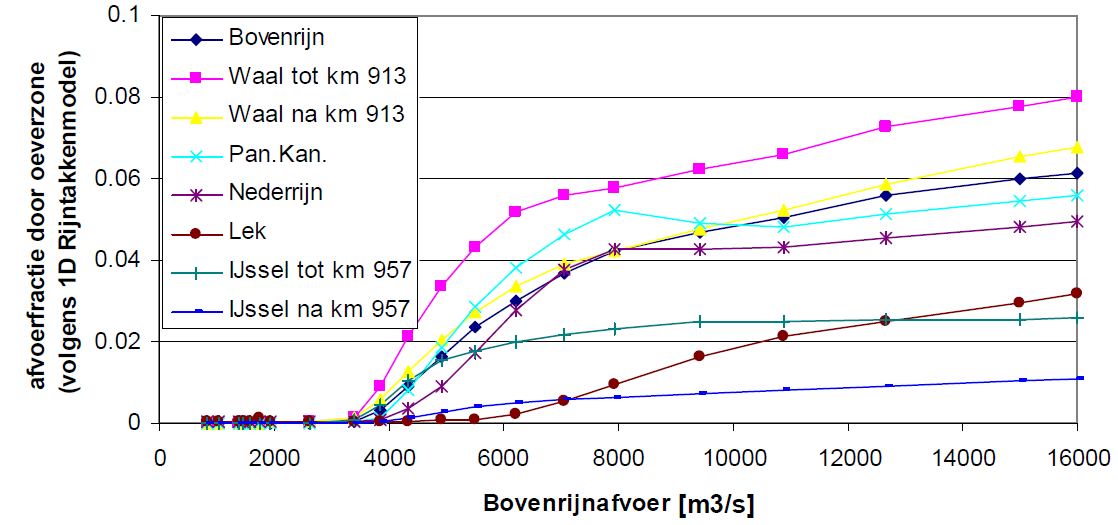
\includegraphics[width=\columnwidth]{figures/Fig2b.png}
\caption{Reach-averaged discharge fraction through the bank zone (based on 1D model of the Rhine branches).}
\label{App.Fig2b}
\end{figure}

These characteristic discharge values can be used to schematize the river hydrograph effectively by means of a limited number of discrete discharge conditions.
Three discharge blocks turn out to be sufficient for many interventions as may bed concluded from \autoref{App.Tab1}.
That is why it has been concluded that \emph{three flow conditions are sufficient to schematize the yearly hydrograph for the purpose of estimating the morphological impact of local interventions}.

\begin{table}
\small
%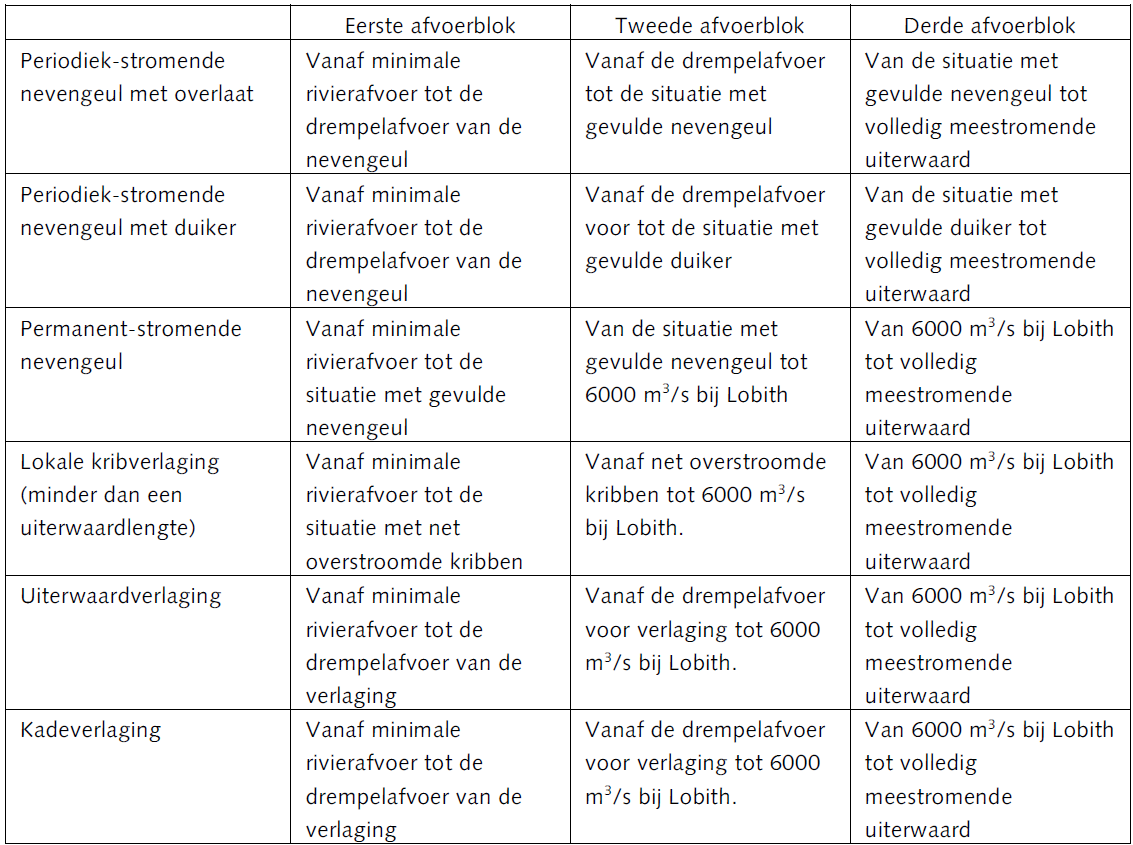
\includegraphics[width=\columnwidth]{figures/Tab1a.png}
\begin{tabular}{p{\columnwidth/4-12pt}|p{\columnwidth/4-12pt}|p{\columnwidth/4-12pt}|p{\columnwidth/4-12pt}}
 & first block & second block & third block \\ \hline
periodically flowing secondary channel with weir & from minimum river flow to minimum discharge for secondary channel & from minimum discharge for secondary channel to bankfull secondary channel & from bankfull secondary channel to fully developed flood plain flow \\ \hline
periodically flowing secondary channel with orifice & from minimum river flow to minimum discharge for secondary channel & from minimum discharge for secondary channel to fully flooded orifice & from fully flooded orifice to fully developed flood plain flow \\ \hline
permanently flowing secondary channel & from minimum river flow to bankfull secondary channel & from bankfull secondary channel to 6000 m\textsuperscript{3}/s at Lobith & from 6000 m\textsuperscript{3}/s at Lobith to fully developed flood plain flow \\ \hline
local lowering of groynes (less than flood plain length) & from minimum river flow to flooded groynes & from flooded groynes to 6000 m\textsuperscript{3}/s at Lobith & from 6000 m\textsuperscript{3}/s at Lobith to fully developed flood plain flow \\ \hline
lowering of the flood plain & from minimum river flow to minimum discharge for new flood plain threshold & from new flood plain threshold to 6000 m\textsuperscript{3}/s at Lobith & from 6000 m\textsuperscript{3}/s at Lobith to fully developed flood plain flow \\ \hline
lowering of levees & from minimum river flow to minimum discharge for new levee threshold & from new levee threshold to 6000 m\textsuperscript{3}/s at Lobith & from 6000 m\textsuperscript{3}/s at Lobith to fully developed flood plain flow \\
\end{tabular}

\caption{Overview of discharge conditions for various interventions in a free flowing Rhine branch.}
\label{App.Tab1}
\end{table}

For a river reach in which water levels (and hence flow conditions) are controlled by means of barriers for a period $T_\text{stuw}$, the minimum river discharge is determined by the river discharge at which the barriers are opened.
\autoref{App.Fig6} shows that the barriers in the Nederrijn are opened at a discharge of 1500 m\textsuperscript{3}/s in the Bovenrijn at Lobith (this value is exceeded during 57 \% of the year) and that the branch is approximately free flowing for discharges above 2200 m\textsuperscript{3}/s in the Bovenrijn at Lobith (exceeded during 33 \% of the year).

\begin{table}
%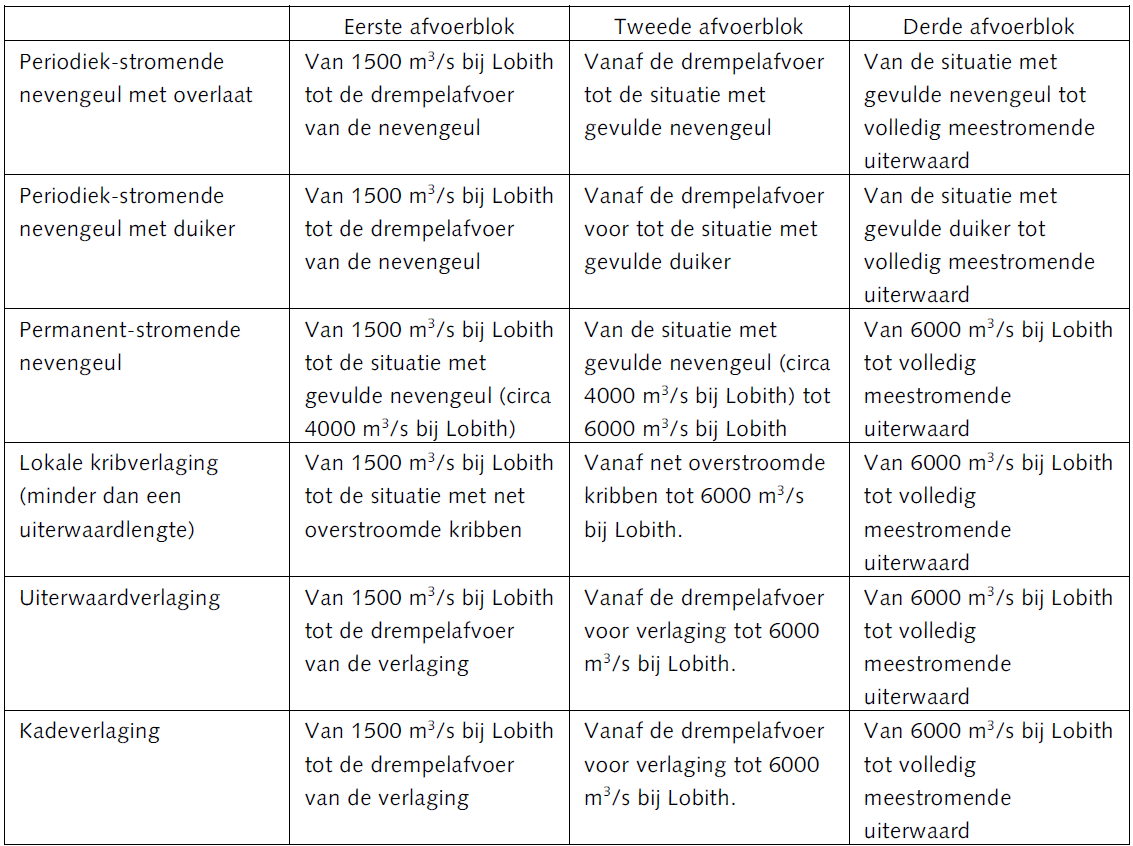
\includegraphics[width=\columnwidth]{figures/Tab1b.png}
\begin{tabular}{p{\columnwidth/4-12pt}|p{\columnwidth/4-12pt}|p{\columnwidth/4-12pt}|p{\columnwidth/4-12pt}}
 & first block & second block & third block \\ \hline
periodically flowing secondary channel with weir & from 1500 m\textsuperscript{3}/s at Lobith to minimum discharge for secondary channel & from minimum discharge for secondary channel to bankfull secondary channel & from bankfull secondary channel to fully developed flood plain flow \\ \hline
periodically flowing secondary channel with orifice & from 1500 m\textsuperscript{3}/s at Lobith to minimum discharge for secondary channel & from minimum discharge for secondary channel to fully flooded orifice & from fully flooded orifice to fully developed flood plain flow \\ \hline
permanently flowing secondary channel & from 1500 m\textsuperscript{3}/s at Lobith to bankfull secondary channel (about 4000 m\textsuperscript{3}/s at Lobith) & from bankfull secondary channel (about 4000 m\textsuperscript{3}/s at Lobith) to 6000 m\textsuperscript{3}/s at Lobith & from 6000 m\textsuperscript{3}/s at Lobith to fully developed flood plain flow \\ \hline
local lowering of groynes (less than flood plain length) & from 1500 m\textsuperscript{3}/s at Lobith to flooded groynes & from flooded groynes to 6000 m\textsuperscript{3}/s at Lobith & from 6000 m\textsuperscript{3}/s at Lobith to fully developed flood plain flow \\ \hline
lowering of the flood plain & from 1500 m\textsuperscript{3}/s at Lobith to minimum discharge for new flood plain threshold & from new flood plain threshold to 6000 m\textsuperscript{3}/s at Lobith & from 6000 m\textsuperscript{3}/s at Lobith to fully developed flood plain flow \\ \hline
lowering of levees & from 1500 m\textsuperscript{3}/s at Lobith to minimum discharge for new levee threshold & from new levee threshold to 6000 m\textsuperscript{3}/s at Lobith & from 6000 m\textsuperscript{3}/s at Lobith to fully developed flood plain flow \\
\end{tabular}

\caption{Overview of discharge conditions for various interventions along the Nederrijn.}
\label{App.Tab2}
\end{table}

\begin{table}
%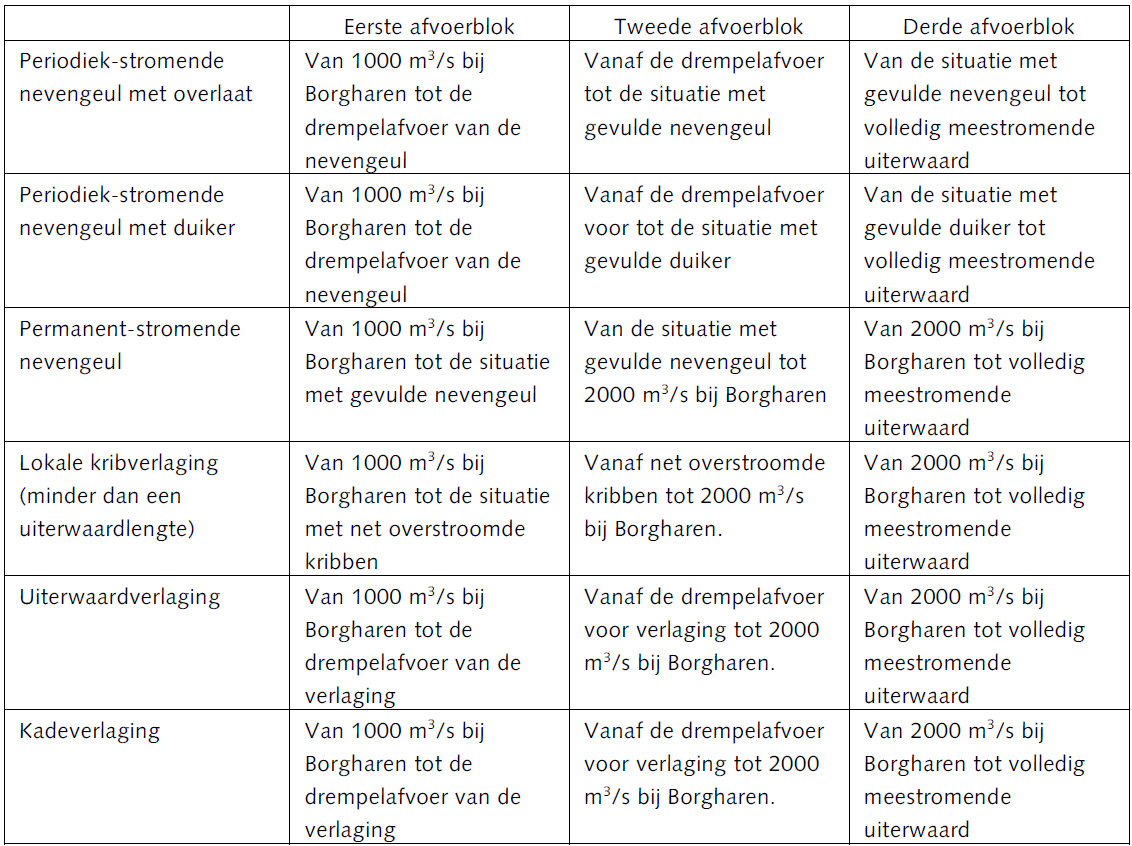
\includegraphics[width=\columnwidth]{figures/Tab1c.png}
\begin{tabular}{p{\columnwidth/4-12pt}|p{\columnwidth/4-12pt}|p{\columnwidth/4-12pt}|p{\columnwidth/4-12pt}}
 & first block & second block & third block \\ \hline
periodically flowing secondary channel with weir & from 1000 m\textsuperscript{3}/s at Borgharen to minimum discharge for secondary channel & from minimum discharge for secondary channel to bankfull secondary channel & from bankfull secondary channel to fully developed flood plain flow \\ \hline
periodically flowing secondary channel with orifice & from 1000 m\textsuperscript{3}/s at Borgharen to minimum discharge for secondary channel & from minimum discharge for secondary channel to fully flooded orifice & from fully flooded orifice to fully developed flood plain flow \\ \hline
permanently flowing secondary channel & from 1000 m\textsuperscript{3}/s at Borgharen to bankfull secondary channel & from bankfull secondary channel to 2000 m\textsuperscript{3}/s at Borgharen & from 2000 m\textsuperscript{3}/s at Borgharen to fully developed flood plain flow \\ \hline
local lowering of groynes (less than flood plain length) & from 1000 m\textsuperscript{3}/s at Borgharen to flooded groynes & from flooded groynes to 2000 m\textsuperscript{3}/s at Borgharen & from 2000 m\textsuperscript{3}/s at Borgharen to fully developed flood plain flow \\ \hline
lowering of the flood plain & from 1000 m\textsuperscript{3}/s at Borgharen to minimum discharge for new flood plain threshold & from new flood plain threshold to 2000 m\textsuperscript{3}/s at Borgharen & from 2000 m\textsuperscript{3}/s at Borgharen to fully developed flood plain flow \\ \hline
lowering of levees & from 1000 m\textsuperscript{3}/s at Borgharen to minimum discharge for new levee threshold & from new levee threshold to 2000 m\textsuperscript{3}/s at Borgharen & from 2000 m\textsuperscript{3}/s at Borgharen to fully developed flood plain flow \\
\end{tabular}

\caption{Overview of discharge conditions for various interventions along the Meuse.}
\label{App.Tab3}
\end{table}

\begin{figure}
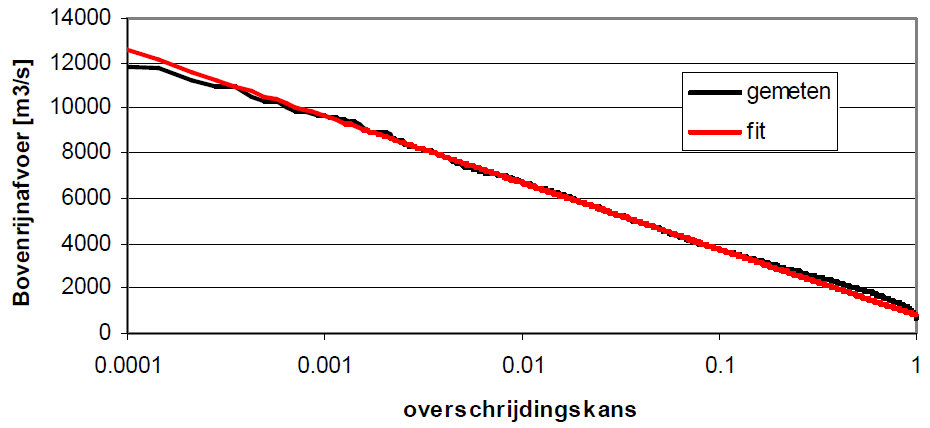
\includegraphics[width=\columnwidth]{figures/Fig3a.png}
\caption{Discharge exceedance curve for the Bovenrijn at Lobith (1970-2000).}
\label{App.Fig3a}
\end{figure}

\begin{figure}
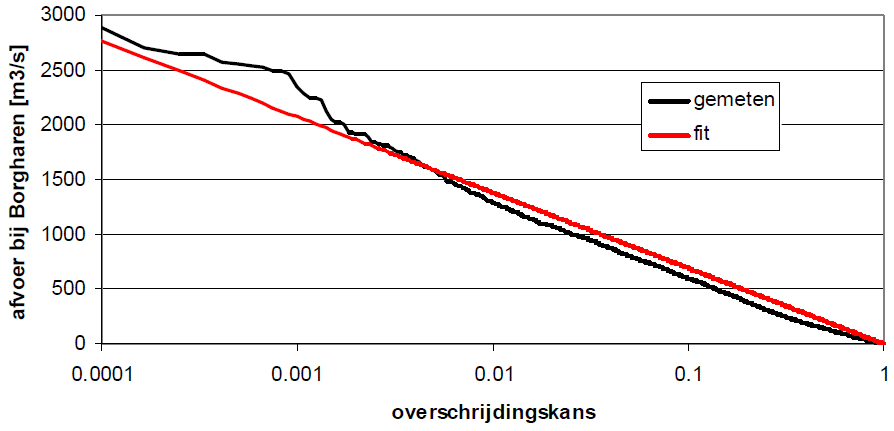
\includegraphics[width=\columnwidth]{figures/Fig3b.png}
\caption{Discharge exceedance curve for the Meuse at Borgharen (1975-2007).}
\label{App.Fig3b}
\end{figure}

In order to quickly estimate the yearly exceedance period for a given discharge, the discharge exceedance curve for the Bovenrijn has been approximated by a curve fitted through the observational data for the period 1970-2000 (\autoref{App.Fig3a}).
The number of days that the discharge $Q_\text{Bovenrijn}$ in the Bovenrijn at lobith is exceeded is given by

\begin{equation}
\label{Eq1a}
T_\text{exceedance, Bovenrijn} = 365 e^{\left ( \frac{800 -  Q_\text{Bovenrijn}}{1280} \right )}
\end{equation}

For the Meuse, in which --- due to imbrication (Grensmaas) and barriers (Zandmaas) --- the higher discharges are more important for the morphological development, the exceedance period for discharges at Borgharen can be estimated as

\begin{equation}
\label{Eq1b}
T_\text{exceedance, Meuse} = 365 e^{\left ( \frac{-  Q_\text{Borgharen}}{300} \right )}
\end{equation}

\subsection{Scientific background of the relaxation model for morphological change}

The rule-of-thumb used to determine the first estimate of the morphological effects within the main channel is based on a highly simplified model of the morphodynamics.
That model and the resulting rule-of-thumb are described in this section.

We start by assuming a quasi-stationary flow pattern and an outflow of discharge and sediment from the main channel while the local water level is independent of the hydraulic and morphological changes in the main channel (a \emph{rigid-lid} approximation).

\begin{figure}
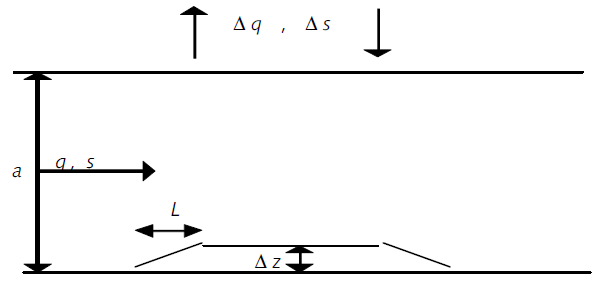
\includegraphics[width=\columnwidth]{figures/Fig4.png}
\caption{Schematic representation of the outflow of water and sediment}
\label{App.Fig4}
\end{figure}

The response of the main channel is represented here by a bed level change $\Delta z_b$ \unitbrackets{m} (raise or lowering) which is small relative to the local water depth.
The mass balance of the water and the sediment in the main channel can be written as
%
\begin{align}
&\text{water} & \pdiff{q_\text{mc}}{s} = -q_\text{out} \label{Eq2} \\
&\text{sediment} & \pdiff{z_b}{t} + \pdiff{s_\text{mc}}{s} = -s_\text{out} \label{Eq3}
\end{align}
%
in which
%
\begin{symbollist}
\item[$q_\text{mc}$] main channel unit discharge \unitbrackets{m\textsuperscript{2}/s}
\item[$q_\text{out}$] \emph{outflow of} unit discharge \emph{to} the flood plain per unit length \unitbrackets{m\textsuperscript{2}/sm}
\item[$s$] streamwise coordinate \unitbrackets{m}
\item[$z_b$] bed level change due to intervention \unitbrackets{m}
\item[$s_\text{mc}$] main channel unit sediment transport including pores \unitbrackets{m\textsuperscript{2}/s}
\item[$s_\text{out}$] \emph{outflow of} unit sediment transport including pores \emph{to} the flood plain per unit length \unitbrackets{m\textsuperscript{2}/sm}
\end{symbollist}

Note that the outflow of sediment is assumed to be a consequence of the outflow of discharge only; the conceptual framework does not allow for selective removal of only sediments.	
The unit sediment transport capacity in the main channel, $s_\text{mc}$, is approximated by $s_\text{mc} = m \left ( q_\text{mc} / h \right )^b$ with $h$ the water depth \unitbrackets{m} in the main channel, $m$ a dimensionless calibration factor and a dimensionless sediment transport exponent $b$ about 5 \citep{Engelundh67}.
Using this approximation the gradients in the sediment transport capacity can be written as
%
\begin{align}
\pdiff{s_\text{mc}}{s} &= m b \left ( \frac{q_\text{mc}}{h} \right )^{b-1} \pdiff{(q_\text{mc} / h)}{s} \\
&= m b \left ( \frac{q_\text{mc}}{h} \right )^{b-1} \left [ \frac{1}{h} \pdiff{q_\text{mc}}{s} - \frac{q_\text{mc}}{h^2} \pdiff{h}{s} \right ] \\
&= b \frac{s_\text{mc}}{q_\text{mc}} \pdiff{q_\text{mc}}{s} - b \frac{s_\text{mc}}{h} \pdiff{h}{s} \\
&\approx b \frac{s_\text{mc}}{q_\text{mc}} \pdiff{q_\text{mc}}{s} + b \frac{s_\text{mc}}{h} \pdiff{z_b}{s}
\label{Eq4}
\end{align}
%
if we assume that the water level gradient is negligible ($\pdiff{z_w}{s} \approx 0$) such that $\pdiff{h}{s} \approx -\pdiff{z_b}{s}$.
Substitution of \autoref{Eq4} into \autoref{Eq3} gives
%
\begin{equation}
\pdiff{z_b}{t} + b \frac{s_\text{mc}}{q_\text{mc}} \pdiff{q_\text{mc}}{s} + b \frac{s_\text{mc}}{h} \pdiff{z_b}{s} = -s_\text{out}
\label{Eq5a}
\end{equation}
%
which after substitution of \autoref{Eq2} in the second term becomes
%
\begin{equation}
\frac{h}{b s_\text{mc}} \pdiff{z_b}{t} + \pdiff{z_b}{s} = h \frac{q_\text{out}}{q_\text{mc}} - h \frac{s_\text{out}}{b s_\text{mc}}
\label{Eq5}
\end{equation}

The dynamic bed level changes will develop starting from the upstream end of the intervention.
The length $L$ over which this sedimentation occurs (i.e.~varies from 0 upstream to maximum amount $\Delta z_b$ downstream) corresponds to the reach over which discharge leaves the main channel and in which the flow pattern is adjusted by the reduced discharge as sketched in \autoref{App.Fig4}.
Hence, this length $L$ may thus be significantly shorter than the length of the intervention or the distance between the inflow and outflow openings of a secondary channel.
The integration of \autoref{Eq5} over this length $L$ results in a relaxation model for the dynamic bed level change due to the intervention
%
\begin{equation}
\frac{h}{b s_\text{mc}} \int_0^L \pdiff{z_b}{t} ds + \int_0^L \pdiff{z_b}{s} ds = \int_0^L \left [ h \frac{q_\text{out}}{q_\text{mc}} - h \frac{s_\text{out}}{b s_\text{mc}} \right ] ds
\label{Eq5a}
\end{equation}
%
\begin{equation}
\frac{h}{b s_\text{mc}} L^* \pdiff{\Delta z_b}{t} + \Delta z_b = - h \frac{\Delta q_\text{mc}}{q_\text{mc}} + h \frac{\Delta s_\text{mc}}{b s_\text{mc}}
\label{Eq5b}
\end{equation}
%
which $\Delta q_\text{mc}$ is the total change in unit discharge in the main channel due to the intervention \unitbrackets{m\textsuperscript{2}/s} and $\Delta s_\text{mc}$ is the total change in unit sediment transport due to the intervention \unitbrackets{m\textsuperscript{2}/s}.
Please note that $q_\text{out}$ was defined above positive for fluxes towards the flood plain, however, the resulting change $\Delta q_\text{mc}$ in the unit discharge within the main channel will be negative for such conditions (equivalently for $s_\text{out}$ and $\Delta s_\text{mc}$); this introduces a sign change on the right hand side.
%
\begin{equation}
\diff{\Delta z_b}{t} = \frac{\Delta z_{b,\text{eq}} - \Delta z_b}{T_m}
\label{Eq5dif}
\end{equation}
%
with a morphological time scale \unitbrackets{s}
%
\begin{equation}
T_m \approx \frac{h L}{b s_\text{mc}}
\label{Eq5T}
\end{equation}
%
and an equilibrium bed level change \unitbrackets{m} given by
%
\begin{equation}
\Delta z_{b,\text{eq}} = -h \left ( \frac{\Delta q_\text{mc}}{q_\text{mc}} - \frac{\Delta s_\text{mc}}{b s_\text{mc}} \right )
\label{Eq6}
\end{equation}
%
This relaxation behaviour can also be observed in the results of the numerical models (both 1D and 2D).

The rule-of-thumb is derived by posing that the bed level change $\Delta z_b$ can be interpreted as the bed level change due to an intervention over a distance $L$ along a stream line starting from the upstream end of the intervention.
The equilibrium value $\Delta z_{b,\text{eq}}$ depends according \autoref{Eq6} on the (original) water depth, the relative change in unit discharge and the relative change in the sediment transport.
The latter term is the result of the sediment flux into the secondary channel which dampens the effect of reduced sediment transport capacity in the main channel.
Ignoring this relatively minor dampening term results in a more conservative estimate.
For interventions over a short distance (i.e.~for the type of interventions for which the rule-of-thumb is applicable) the water level changes are an order of magnitude smaller than the bed level changes.
Therefore, one can rewrite \autoref{Eq6} to state that the equilibrium bed level change $\Delta z_{b,\text{eq}}$ equals the product of the water depth and the relative change in the main channel velocity $u$ \unitbrackets{m/s}:
%
\begin{equation}
\Delta z_{b,\text{eq}} \approx -h \left ( \frac{\Delta u}{u} \right )
\label{Eq6v2}
\end{equation}
%
A similar result can be obtained for graded bed material (sand/gravel mixtures) if it's assumed that the individual sediment fractions don't influence each other's mobility (Appendix C in \citet{Waterdienst2008}).
Such an assumption is valid at sufficiently high bed shear stresses, such as during flood conditions.

\subsection{The relaxation model applied to seasonal variability}

The bed level development during a relaxation period is (as a solution of \autoref{Eq5dif}) given by
%
\begin{equation}
z_{b,i} = z_{b,i} (0) + [z_{b,i,\text{eq}} - z_{b,i}(0)](1 - e^{-t/T_{m,i}})
\label{Eq7}
\end{equation}
%
with
%
\begin{symbollist}
\item[$z_{b,i}$] \unitbrackets{m} the morphological effect of the intervention during period $i$
\item[$z_{b,i}(0)$] \unitbrackets{m} the morphological effect at the start of period $i$
\item[$z_{b,i,\text{eq}}$] \unitbrackets{m} the equilibrium effect of the intervention during period $i$
\item[$t$] \unitbrackets{day} time
\item[$T_{m,i}$] \unitbrackets{day} the morphological time scale during period $i$
\end{symbollist}

\begin{figure}
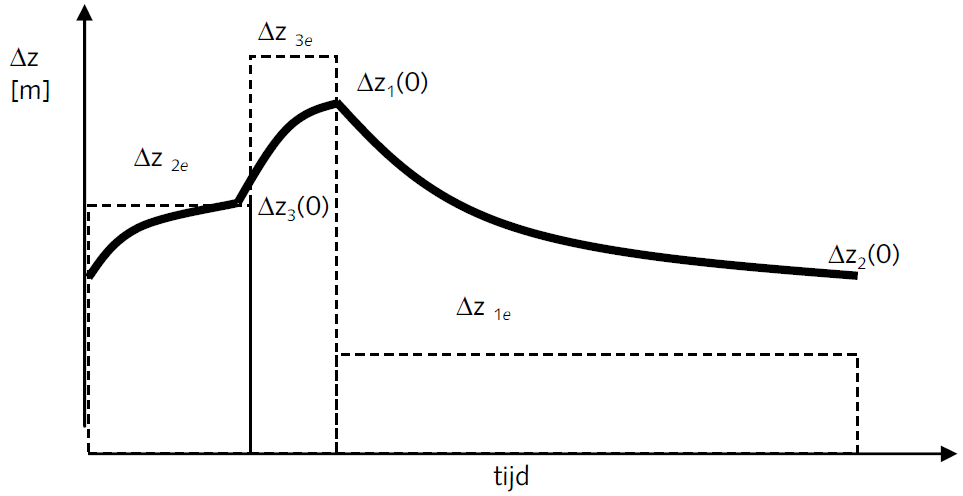
\includegraphics[width=\columnwidth]{figures/Fig5.png}
\caption{Schematic maximum bed level changes at the upstream end.}
\label{App.Fig5}
\end{figure}

\autoref{Eq7} implies that at the end of period $i$ (lasting for a period of $T_i$ days) the morphological effect of the intervention is given by
%
\begin{equation}
z_{b,i+1}(0) = z_{b,i} (0) \sigma_i + z_{b,i,\text{eq}} (1-\sigma_i) \text{ with } \sigma_i = e^{-T_i/T_{m,i}}
\label{Eq8a}
\end{equation}

If the yearly hydrograph is schematized using three periods, one obtains the following set of three equations for the three periods by assuming periodicity (the final bed level of the third period equals the initial bed level of the first period)
%
\begin{align}
z_{b,2}(0) &= z_{b,1}(0) \sigma_1 + z_{b,1,\text{eq}} (1-\sigma_1) \label{Eq8b} \\
z_{b,3}(0) &= z_{b,2}(0) \sigma_2 + z_{b,2,\text{eq}} (1-\sigma_2) \label{Eq8c} \\
z_{b,1}(0) &= z_{b,3}(0) \sigma_3 + z_{b,3,\text{eq}} (1-\sigma_3) \label{Eq8d}
\end{align}

We can solve these three equations for the unknown bed levels $z_{b,1}(0)$, $z_{b,2}(0)$ and $z_{b,3}(0)$.
This gives the following three expressions
%
\begin{align}
z_{b,1}(0) &= \frac{z_{b,1,\text{eq}} (1-\sigma_1) \sigma_2 \sigma_3 + z_{b,2,\text{eq}} (1-\sigma_2) \sigma_3 + z_{b,3,\text{eq}} (1-\sigma_3)}{1 - \sigma_1 \sigma_2 \sigma_3} \label{Eq8e} \\
z_{b,2}(0) &= \frac{z_{b,1,\text{eq}} (1-\sigma_1) + z_{b,2,\text{eq}} (1-\sigma_2) \sigma_3 \sigma_1 + z_{b,3,\text{eq}} (1-\sigma_3) \sigma_1}{1 - \sigma_1 \sigma_2 \sigma_3} \label{Eq8f} \\
z_{b,3}(0) &= \frac{z_{b,1,\text{eq}} (1-\sigma_1) \sigma_2 + z_{b,2,\text{eq}} (1-\sigma_2) + z_{b,3,\text{eq}} (1-\sigma_3) \sigma_1 \sigma_2}{1 - \sigma_1 \sigma_2 \sigma_3} \label{Eq8g}
\end{align}

The lower bound for the morphological impact of the intervention will be equal to $\min[z_{b,1}(0), z_{b,2}(0), z_{b,3}(0)]$ and the upper bound is given by $\max[z_{b,1}(0), z_{b,2}(0), z_{b,3}(0)]$.
For the schematized hydrograph shown in \autoref{App.Fig5} the bed level change is

\begin{itemize}
\item maximum at $z_{b,1}(0)$ (\autoref{Eq8e}) after flood period 3 (the third block in \autoref{App.Tab2})
\item minimum at $z_{b,2}(0)$ (\autoref{Eq8f}) after the low flow period 1 (the first block in \autoref{App.Tab2}).
\end{itemize}

In case the river section is experiences nearly stagnant flow conditions due to barriers a yearly period without bed level changes is inserted between low flow period 1 and the transitional flow period 2.\footnote{Earlier versions of this manual suggested that this period might be inserted between the flood period 3 and the low flow period 1, but algorithmically it was always placed between periods 1 and 2.}

We can't only obtain expressions for the two extreme (minimum, maximum) values but we can also determine an expression for the year-averaged bed level change by integrating \autoref{Eq7} per constant discharge period to
%
\begin{align}
\bar{z}_{b,i} &= \frac{1}{T_i} \int_0^{T_i}{z_{b,i} (0) + [z_{b,i,\text{eq}} - z_{b,i}(0)](1 - e^{-t/T_{m,i}})}dt \\
&= \frac{1}{T_i} \left . \left ( {z_{b,i,\text{eq}} t + [z_{b,i,\text{eq}} - z_{b,i}(0)]T_{m,i} e^{-t/T_{m,i}}} \right ) \right |_{t=0}^{t=T_i} \\
&= z_{b,i,\text{eq}} + [z_{b,i,\text{eq}} - z_{b,i}(0)] \frac{T_{m,i}}{T_i} ( e^{-T_i/T_{m,i}} - 1 )
\end{align}
%
and over all periods to
%
\begin{equation}
\bar{z}_b = \frac{\sum{z_{b,i,\text{eq}} T_i}}{\sum{T_i}} + \frac{\sum{(z_{b,i,\text{eq}}-z_{b,i}(0)) T_{m,i} (\sigma_i-1)}}{\sum{T_i}}
\label{Eq8h}
\end{equation}
%
If all bed level changes are removed after the flood period by means of dredging, the yearly dredging amount can finally be estimated by ignoring any excess depth.
After all, the maximum bed level change at the end of the flood season can with $z_{b,1}(0) = 0$ and \autoref{Eq8a} to \autoref{Eq8i} be expressed as the maximum dredging depth $z_\text{mdd}$

\begin{equation}
z_\text{mdd} = z_{b,1,\text{eq}}(1-\sigma_1) \sigma_2 \sigma_3 + z_{b,2,\text{eq}} (1-\sigma_2) \sigma_3 + z_{b,3,\text{eq}} (1-\sigma_3)
\label{Eq8i}
\end{equation}

Because this estimated doesn't take into account the sediment supply by the river, \autoref{Eq8i} can overestimate the maintenance dredging required.
\autoref{Eq8i} is therefore not included in the \dfastmi analysis.

\subsection{Estimate of the spatial distribution of the bed level changes}

\autoref{Eq8e} gives the maximum and \autoref{Eq8f} gives the minimum bed level change at the upstream end of the intervention.
Moving downstream for that point, the bed level change consists of a minimum bed level change $z_{b,1,\text{eq}}$ plus the part of the flood deposit that moves downstream during low flow conditions.
During a flood the downstream migrating sedimentation volume may temporarily even cause bed level changes larger than $z_{b,2,\text{eq}}$ but this is rather unlikely.
For convenience, it's therefore assumed that the maximum and minimum bed level change given by \autoref{Eq8e} and \autoref{Eq8f} are valid \emph{for each individual point in the main channel within the impacted area}.

This approximation implies that first the values of $z_{b,1,\text{eq}}$, $z_{b,2,\text{eq}}$ and $z_{b,3,\text{eq}}$ can be determined for every computational cell of the simulation in the main channel.
Subsequently the minimum (at the end of the low flow period) and maximum bed level change (at the end of the flood period) can be estimated given the approximated values for $\sigma_1$, $\sigma_2$ and $\sigma_3$ and \autoref{Eq8f} and \autoref{Eq8e} respectively.

\subsection{Time scales for bed level change}

The magnitude of the maximum bed level change at the end of the flood period and the minimum bed level change at the end of the low flow period both depend on the morphological time scales $T_{m,i}$ \unitbrackets{day} which define the rate of response of the bed levels.
Using \autoref{Eq5T} the time scale $T_{m,i}$ can also be written as $T_{m,i} = L/w_i$ with $w_i$ the bed celerity, i.e.~the propagation speed of bed level changes, and $L$ the distance intervention along the flow direction over which the bed level changes are accumulated.
As mentioned before, the length $L$ corresponds to the distance over which flow leaves the main channel and the flow pattern in the main channel adjusts to the reduced discharge.
Obviously, this distance varies in reality over the channel width and it depends on the discharge condition considered.
For consistent use of the rule-of-thumb, it's assumed that the length $L$ corresponds to twice the main channel width $B_\text{mc}$.

The second parameter in the definition of the morphological time scale is the bed celerity.
Based on statistics of width-averaged bed level observations averaged per km chainage year-averaged values have been determined \citep{RIZA2005} for the Dutch rivers.
These values are presented in \autoref{App.Tab2} and \autoref{App.Tab3} for Rhine branches and Meuse respectively.

\begin{table}
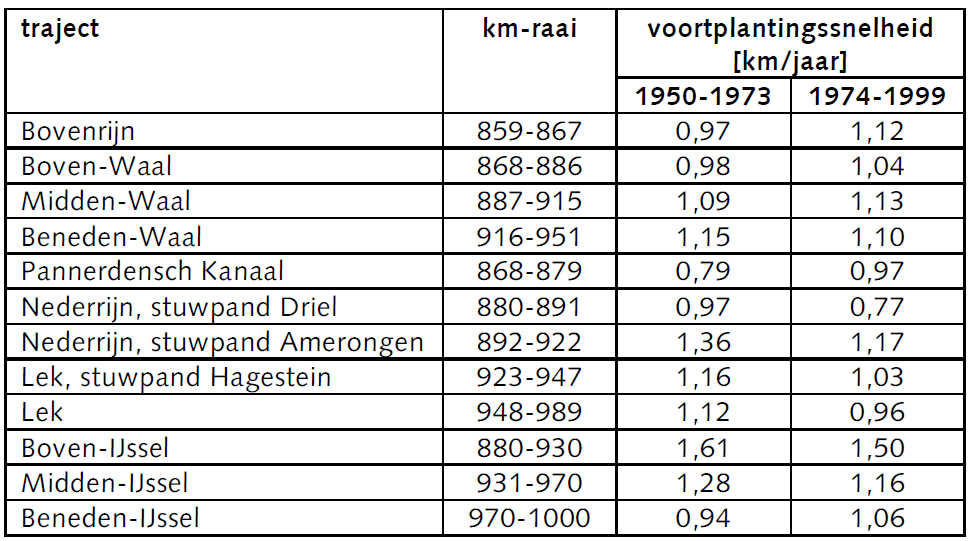
\includegraphics[width=\columnwidth]{figures/Tab2.png}
\caption{Overview of average bed celerities (based on km-averaged bed levels including the effects of dredging) by \citet{RIZA2005}.}
\label{App.Tab2Again}
\end{table}

\begin{table}
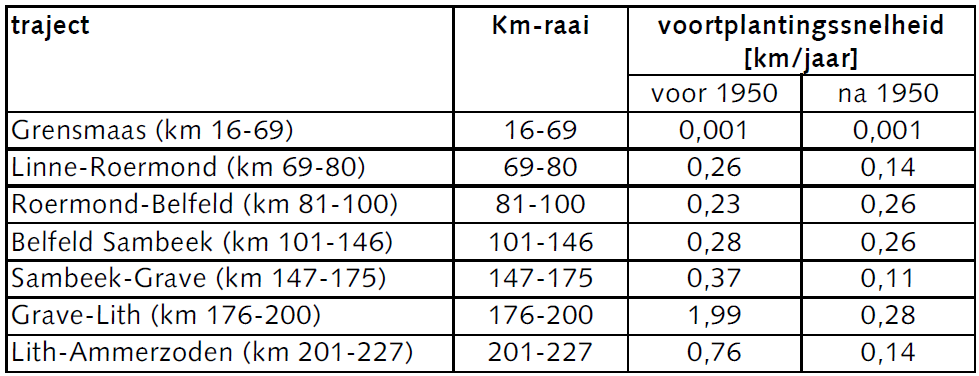
\includegraphics[width=\columnwidth]{figures/Tab3.png}
\caption{Overview of the reach averaged bed celerities (based on km-averaged bed levels including the effects of dredging) by \citet{Waterdienst2008}.}
\label{App.Tab3Again}
\end{table}

\begin{table}
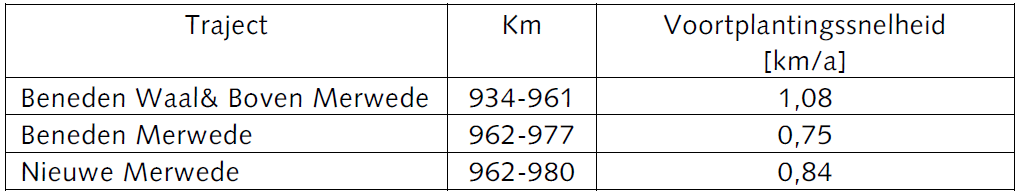
\includegraphics[width=\columnwidth]{figures/Tab4.png}
\caption{Overview of the reach averaged bed celerities (based on km-averaged bed levels for the period 1975-2000 including the effects of dredging) by \citet{RIZA2007}.}
\label{App.Tab4}
\end{table}

In order to translate these empirical year averaged values to discrete values per discharge block the following approximation is used for free flowing Rhine branches.
For the Bovenrijn discharges which are predominantly larger than 4000 m\textsuperscript{3}/s (during on average 8 \% of the year) a "high flow bed celerity" $w_h$ of 10 m/dag (3.65 km/yr) is used.

For discharge blocks which are predominantly below 4000 m\textsuperscript{3}/s a "low flow bed celerity" $w_l$ is used which is derived from the year-averaged bed celerity $\bar{c}$ as

\begin{equation}
w_l = \frac{\bar{c} - 0.082 \cdot 365}{0.918}
\label{Eq9}
\end{equation}

However, this approximation \autoref{Eq9} is only valid for the free flowing Rhine branches, hence it's for instance not valid for the Nederrijn where at low discharges the barriers are closed (\autoref{App.Fig6}).

\begin{figure}
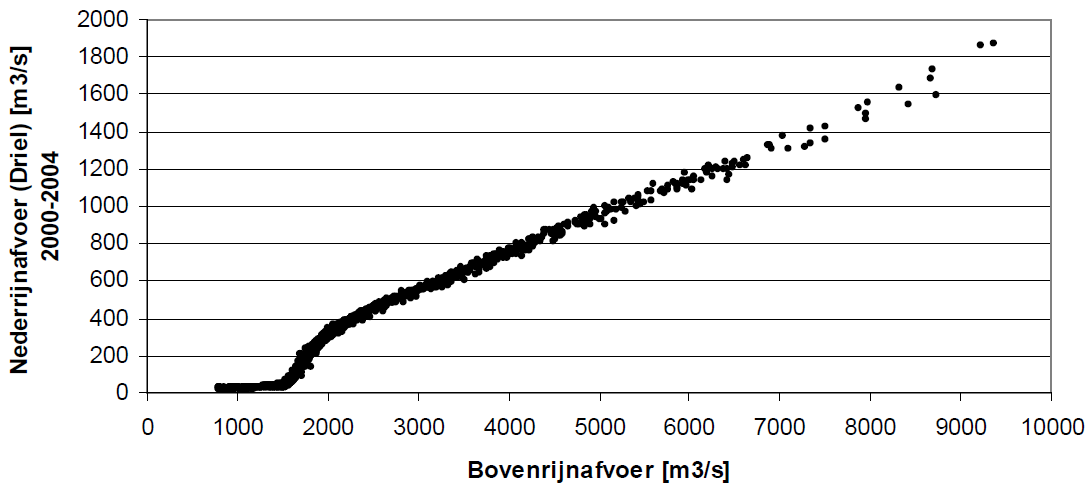
\includegraphics[width=\columnwidth]{figures/Fig6.png}
\caption{Nederrijn discharges at Driel-boven based on Donar database for the period 2000-2004).}
\label{App.Fig6}
\end{figure}

\autoref{App.Fig6} shows that the barriers in the Nederrijn are opened at a discharge of 1500 m\textsuperscript{3}/s in the Bovenrijn at Lobith (this value is exceeded during 57 \% of the year) and that the branch is approximately free flowing for discharges above 2200 m\textsuperscript{3}/s in the Bovenrijn at Lobith (exceeded during 33 \% of the year).
It's therefore assumed that the year-averaged bed celerity related to the low and high flow values as $\bar{c} = 0.082 w_h + (0.918 - 0.33) w_l$ such that for $w_h = 3,65$ km/yr we obtain

\begin{equation}
w_l = \frac{\bar{c} - 0.082 \cdot 3.65}{0.918 - 0.33}
\label{Eq10a}
\end{equation}

For the Meuse the we apply the following approximation.
It's assumed that the Meuse barriers are open for on average 10 days per year (3 \% of the time) such that the bed celerity can be estimated as

\begin{equation}
w_h = \frac{\bar{c}}{0.03}
\label{10b}
\end{equation}


Finally, due to the gradation the river bed of the Grensmaas will only become mobile at discharges above 1000 m\textsuperscript{3}/s which occurs on average about 4 days a year.
The bed celerity is thus estimated as

\begin{equation}
w_h = \frac{\bar{c}}{0.01}
\label{Eq10c}
\end{equation}

Based on the approximations \autoref{Eq9} to \autoref{Eq10c} and the year-averaged bed celerity values in \autoref{App.Tab2Again} to \autoref{App.Tab4} we obtain estimates for the bed celerities during high and low flow conditions.

\begin{table}
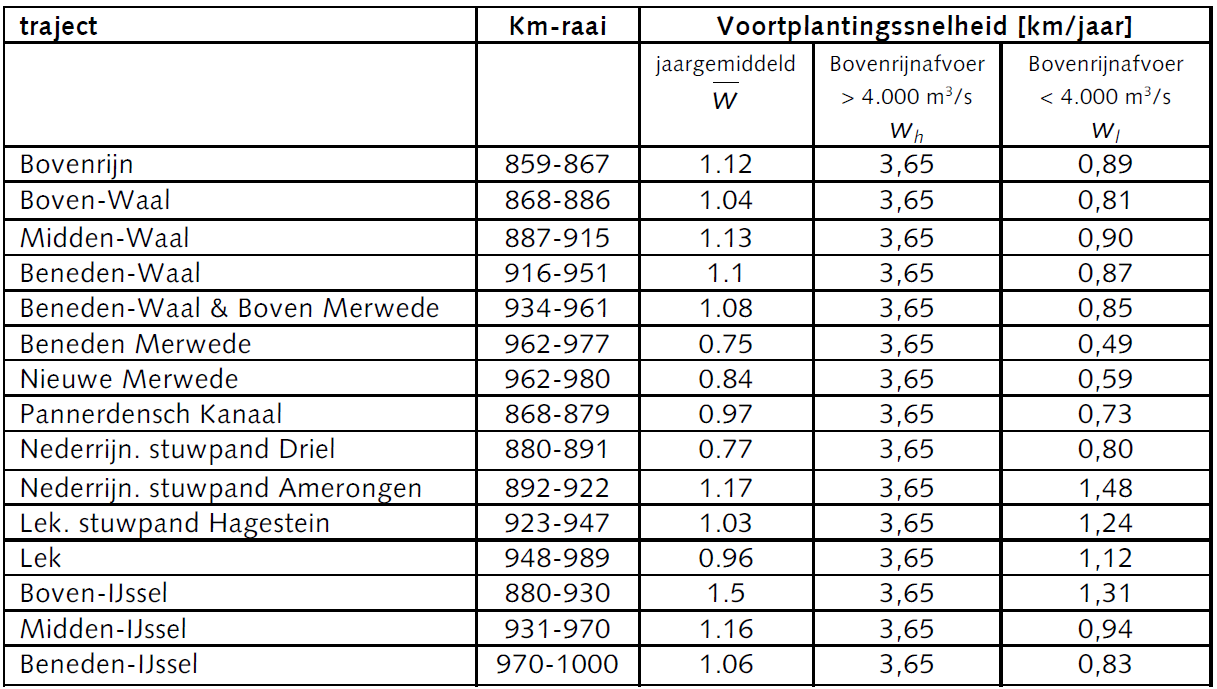
\includegraphics[width=\columnwidth]{figures/Tab4_the2nd.png}
\caption{Representative bed celerities during high- and low-flow conditions Rhine branches.}
\label{App.Tab4RT}
\end{table}

\begin{table}
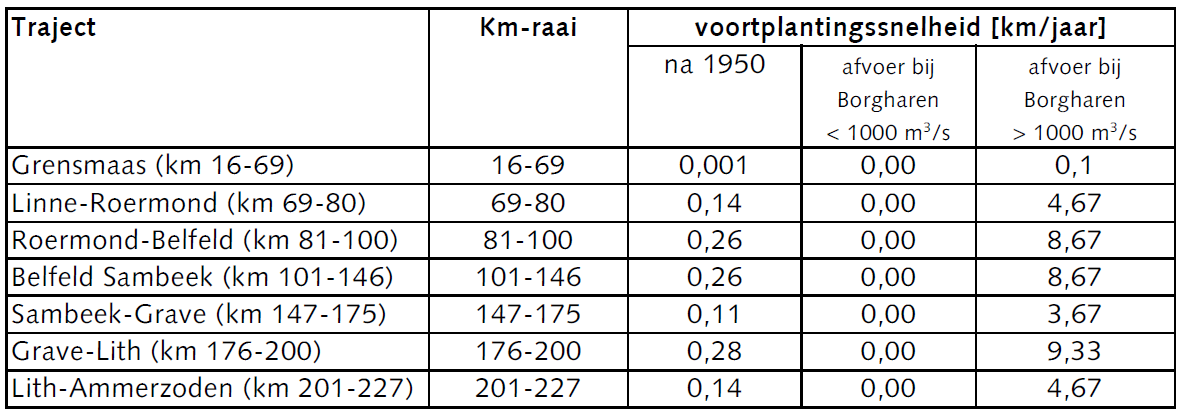
\includegraphics[width=\columnwidth]{figures/Tab5.png}
\caption{Representative bed celerities during high- and low-flow conditions Meuse.}
\label{App.Tab5}
\end{table}


\section{Steps in the analysis}

To apply the rule-of-thumb one should carry out the following five steps.
\dfastmi can perform steps 2 and 4 for you (except for the computation of $z_\text{mdd}$).

\begin{enumerate}
\item Characterize the intervention to be evaluated using \dfastmi

\begin{itemize}
\item Determine the threshold discharge $Q_\text{thr}$ (at Lobith/Borgharen) at which the intervention (indirectly) starts to influence the flow pattern in the main channel.

\item Determine the bankfull discharge $Q_\text{bf}$ (at Lobith/Borgharen) at which the intervention is fully flooded (bankfull flow)
\end{itemize}

\item Define the discharge blocks (block 1 "low flow", block 3 "flood" and block 2 "transitional between low and flood flows") using

\begin{itemize}
\item \autoref{App.Tab7} for the Rhine branches
\item \autoref{App.Tab8} for the Meuse
\end{itemize}

\item Perform the (up to six) necessary hydrodynamic simulations

\item Compute the characteristic bed level change per grid point in the main channel

\begin{itemize}
\item maximum value \unitbrackets{m} at the end of the flood season

\begin{equation}
z_{b,1}(0) = \frac{z_{b,1,\text{eq}} (1-\sigma_1) \sigma_2 \sigma_3 + z_{b,2,\text{eq}} (1-\sigma_2) \sigma_3 + z_{b,3,\text{eq}} (1-\sigma_3)}{1 - \sigma_1 \sigma_2 \sigma_3}
\end{equation}

\item minimum value \unitbrackets{m} at the end of the low flow season

\begin{equation}
z_{b,2}(0) = \frac{z_{b,1,\text{eq}} (1-\sigma_1) + z_{b,2,\text{eq}} (1-\sigma_2) \sigma_3 \sigma_1 + z_{b,3,\text{eq}} (1-\sigma_3) \sigma_1}{1 - \sigma_1 \sigma_2 \sigma_3}
\end{equation}

\item transitional value \unitbrackets{m} at the end of the transition block before the flood period

\begin{equation}
z_{b,3}(0) = \frac{z_{b,1,\text{eq}} (1-\sigma_1) \sigma_2 + z_{b,2,\text{eq}} (1-\sigma_2) + z_{b,3,\text{eq}} (1-\sigma_3) \sigma_1 \sigma_2}{1 - \sigma_1 \sigma_2 \sigma_3}
\end{equation}

\item year-averaged value \unitbrackets{m}

\begin{equation}
z_{b,m} = T_1 z_{b,1}(0) + T_2 z_{b,2}(0) + T_3 z_{b,3}(0)
\end{equation}

\item the maximum dredging depth (ignoring any excess depth)

\begin{equation}
z_\text{mdd} = z_{b,1,\text{eq}} (1-\sigma_1) \sigma_2 \sigma_3 + z_{b,2,\text{eq}} (1-\sigma_2) \sigma_3 + z_{b,3,\text{eq}} (1-\sigma_3)
\end{equation}
\end{itemize}

\item{Visualize the characteristic bed level changes in a graph or on a map}

\end{enumerate}

\begin{table}
\caption{Definition of discharge blocks for the Rhine branches}
\label{App.Tab7}
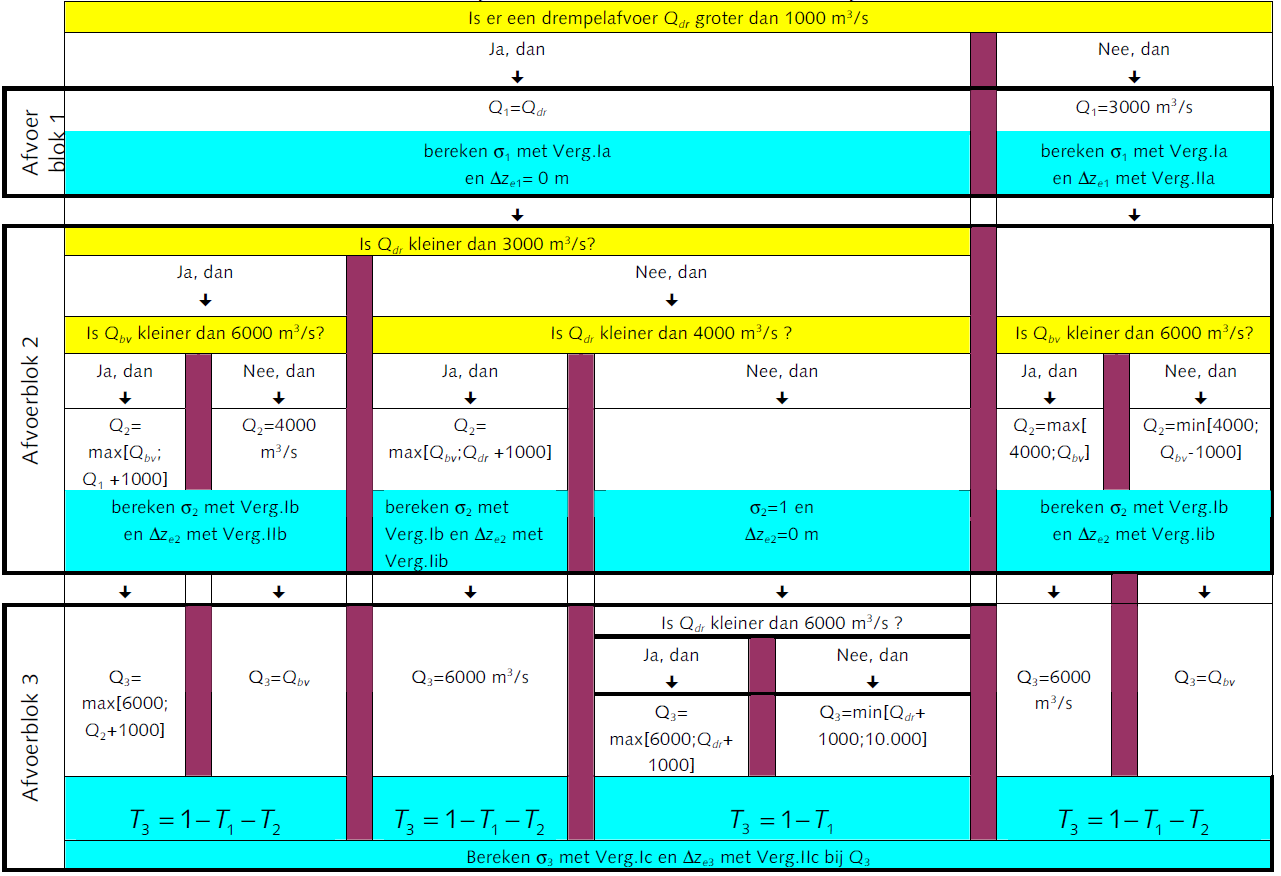
\includegraphics[width=\columnwidth]{figures/Tab7.png}
%
\begin{equation}
\sigma_1 = e^{-\frac{w_l}{2 B_n} T_1}
\end{equation}
with $T_1 = e^{\left ( \frac{800-Q_\text{bar}}{1280} \right )} - e^{\left ( \frac{800-Q_1}{1280} \right )}$ and $w_l$ from \autoref{App.Tab4RT} (with $Q_\text{bar} = 1500$ m\textsuperscript{3}/s for Nederrijn and Lek and $Q_\text{stuw} = 800$ m\textsuperscript{3}/s for the other branches)
%
\begin{equation}
\sigma_2 = e^{-\frac{w_h}{2 B_n} T_2}
\end{equation}
%
\begin{equation}
\sigma_3 = e^{-\frac{w_h}{2 B_n} T_3}
\end{equation}
with $T_2 = e^{\left ( \frac{800-Q_1}{1280} \right )} - e^{\left ( \frac{800-Q_2}{1280} \right )}$ and $w_h$ from \autoref{App.Tab4RT}.
%
\begin{equation}
\Delta z_{b,1,\text{eq}} = -h_o \frac{u_n - u_o}{u_o} \text{  for $Q_1$}
\end{equation}
%
\begin{equation}
\Delta z_{b,2,\text{eq}} = -h_o \frac{u_n - u_o}{u_o} \text{  for $Q_2$}
\end{equation}
%
\begin{equation}
\Delta z_{b,3,\text{eq}} = -h_o \frac{u_n - u_o}{u_o} \text{  for $Q_3$}
\end{equation}
based on reference water depths $h_o$ and velocities $u_o$ and modified velocities $u_n$ from the simulations.
\end{table}


\begin{table}
\caption{Definition of discharge blocks for the Meuse}
\label{App.Tab8}
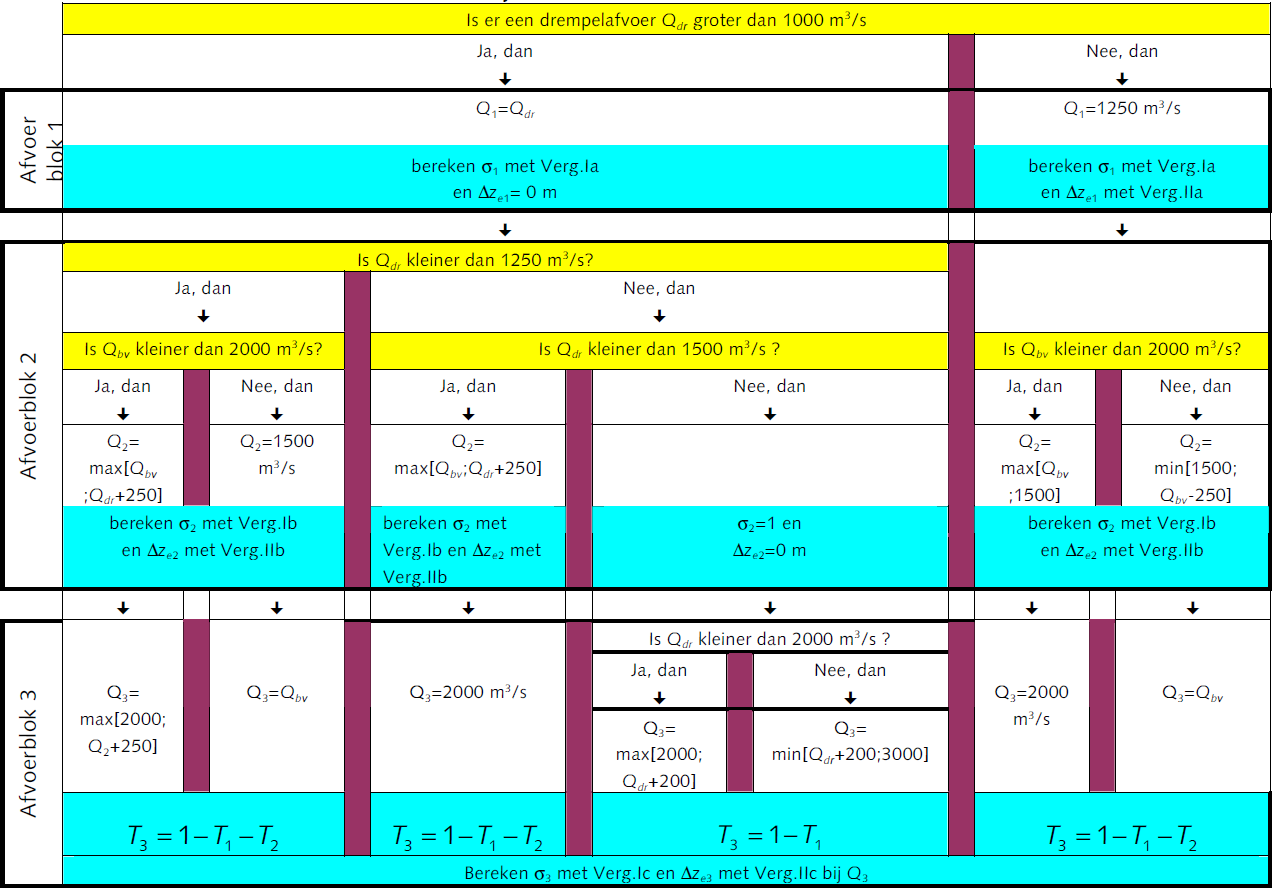
\includegraphics[width=\columnwidth]{figures/Tab8.png}
%
\begin{equation}
\sigma_1 = e^{-\frac{w_l}{2 B_n} T_1}
\end{equation}
with $T_1 = e^{\left ( - \frac{Q_\text{bar}}{300} \right )} - e^{\left ( - \frac{Q_1}{300} \right )}$; $Q_\text{bar} = 100$ m\textsuperscript{3}/s and $w_l$ from \autoref{App.Tab5}.
%
\begin{equation}
\sigma_2 = e^{-\frac{w_h}{2 B_n} T_2}
\end{equation}
%
\begin{equation}
\sigma_3 = e^{-\frac{w_h}{2 B_n} T_3} \text{ with $w_h$ from \autoref{App.Tab8}}
\end{equation}
 with $T_2 = e^{\left ( - \frac{Q_1}{300} \right )} - e^{\left ( - \frac{Q_2}{300} \right )}$ and $w_h$ from \autoref{App.Tab5}.
%
\begin{equation}
\Delta z_{b,1,\text{eq}} = -h_o \frac{u_n - u_o}{u_o} \text{  for $Q_1$}
\end{equation}
%
\begin{equation}
\Delta z_{b,2,\text{eq}} = -h_o \frac{u_n - u_o}{u_o} \text{  for $Q_2$}
\end{equation}
%
\begin{equation}
\Delta z_{b,3,\text{eq}} = -h_o \frac{u_n - u_o}{u_o} \text{  for $Q_3$}
\end{equation}
based on reference water depths $h_o$ and velocities $u_o$ and modified velocities $u_n$ from the simulations.

The premisses are: the flow in the main channel is well developed at $Q = 1000$ m\textsuperscript{3}/s, and at $Q = 2000$ m\textsuperscript{3}/s the flows in main channel and floodplain are both well developed.
\end{table}


\section{Examples}

This section describes three examples of how \dfastmi version 2 could be used.

\subsection{Example 1: secondary channel along the Waal}

For this (manually analyzed) case the effect of the secondary channel was analyzed by means of the results of a 1D \sobek model instead of 2D WAQUA or \dflowfm simulation results.
The secondary channel is located along the Waal river at chainage 900-905 km.
The secondary channel was represented in the 1D Rijntakken model as a local lateral extraction of river discharge.
The extraction was 3 \% of the total river discharge up to 4000 m\textsuperscript{3}/s beyond that the discharge increases linearly up to 10 \% at 7000 m\textsuperscript{3}/s and higher discharges.
The effect on the main channel discharge is shown for a number of characteristic cross-sectional profiles in \autoref{App.Fig7}.
The changes in the \emph{main channel} discharge caused by the secondary channel do not simply follow from the relationship between the secondary channel discharge and the \emph{total} river discharge.
After all, the secondary channel also lowers the water level which introduces a non-linear effect in particular in the lower range of the flood discharges.
As a result the \emph{main channel} discharge does not decrease proportionally to the extra flow area added by the secondary channel (e.g.~at the profile at km 900.5 at Bovenrijn discharges between 7000 and 8000 m\textsuperscript{3}/s).

\begin{figure}
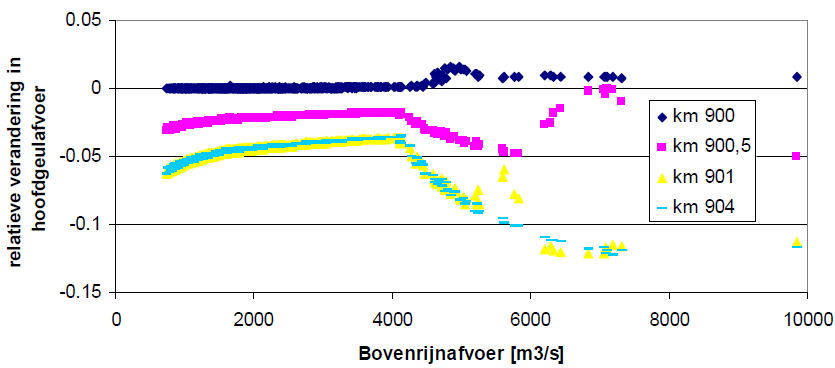
\includegraphics[width=\columnwidth]{figures/Fig7.png}
\caption{Influence of a secondary channel on the main channel discharge of the Waal}
\label{App.Fig7}
\end{figure}

\subsubsection*{Step 1) Characterize the intervention}

The secondary channel removes 3 \% of the total discharge for all discharges below 4000 m\textsuperscript{3}/s in the Bovenrijn.
Above that value the withdrawal increases linearly up to 10 \% at 7000 m\textsuperscript{3}/s.
There is no threshold discharge for the secondary channel: it is active at all discharges.
The secondary channel reaches bankfull at a river discharge of 4000 m\textsuperscript{3}/s.

\subsubsection*{Step 2) Define the discharge blocks}

Because there is no threshold discharge the discharge $Q_1 = 3000$ m\textsuperscript{3}/s is used for the first (low flow) block.
For the second block (transitional discharges) applies that the secondary channel reaches bankfull at 4000 m\textsuperscript{3}/s, so $Q_2 = 4000$ m\textsuperscript{3}/s.
The discharge $Q_3$ of the third block (flood) is in agreement with \autoref{App.Tab7} equal to 6000 m\textsuperscript{3}/s.
These values can be used to compute the relative duration of each block as

\begin{itemize}
\item $Q_1=3000$ m\textsuperscript{3}/s implies $T_1 = 1-e^{\frac{800-3000}{1280}} = 0.84$
\item $Q_2=4000$ m\textsuperscript{3}/s implies $T_2 = e^{\frac{800-3000}{1280}} - e^{\frac{800-4000}{1280}} = 0.09$
\item $Q_3=6000$ m\textsuperscript{3}/s implies $T_3 = 1-T_1-T_2 = 0.07$
\end{itemize}

\subsubsection*{Step 3) Equilibrium bed level changes}

For each of the three characteristic discharges the equilibrium bed level changes were determined for each relevant cross-sectional profile based on the \sobek results as

\begin{equation}
\Delta z_{b,i,\text{eq}} = -h_o \frac{Q_{\text{main channel},n} - Q_{\text{main channel},o}}{Q_{\text{main channel},o}}
\end{equation}

\Note Usually the results of a 2D model are used for each individual computational point in the main channel.
However, for this application based on \sobek results the total main channel discharge and the average main channel depth were used which thus only verifies the impact along a single stream path.

The resulting equilibrium values are shown in \autoref{App.Fig8}.

\begin{figure}
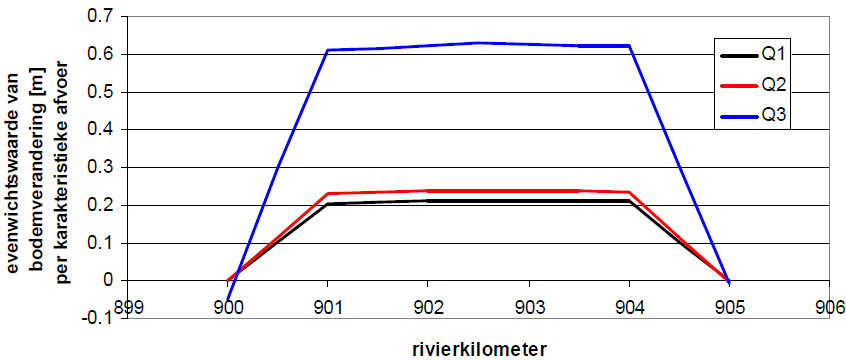
\includegraphics[width=\columnwidth]{figures/Fig8.png}
\caption{Equilibrium bed level changes in the main channel of the Waal at the site of the secondary channel.}
\label{App.Fig8}
\end{figure}

\subsubsection*{Step 4) Time scales for relaxation}

The main channel width (normal width between groyne heads) at the site of the secondary channel is 260 m.
The bed celerity for low discharges is 900 m/yr; for high discharges this increases to 3650 m/yr.
Consequently, for each block we can compute

\begin{align}
\sigma_1 &= e^{-\frac{w_l}{2B_n}T_1} = e^{-\frac{900}{2 \cdot 260} 0.84} = 0.18 \\
\sigma_2 &= e^{-\frac{w_l}{2B_n}T_2} = e^{-\frac{3650}{2 \cdot 260} 0.09} = 0.73 \\
\sigma_3 &= e^{-\frac{w_l}{2B_n}T_3} = e^{-\frac{3650}{2 \cdot 260} 0.07} = 0.78
\end{align}

\subsubsection*{Step 5) Computation of the characteristic bed level changes}

Based on the equilibrium values determined in step 3 and the relaxation factors of step 4 the characteristic bed level changes can be computed using

\begin{align}
z_{b,1}(0) &= \frac{z_{b,1,\text{eq}} (1-\sigma_1) \sigma_2 \sigma_3 + z_{b,2,\text{eq}} (1-\sigma_2) \sigma_3 + z_{b,3,\text{eq}} (1-\sigma_3)}{(1 - \sigma_1 \sigma_2 \sigma_3} \\
z_{b,2}(0) &= \frac{z_{b,1,\text{eq}} (1-\sigma_1) + z_{b,2,\text{eq}} (1-\sigma_2) \sigma_3 \sigma_1 + z_{b,3,\text{eq}} (1-\sigma_3) \sigma_1}{1 - \sigma_1 \sigma_2 \sigma_3}
\end{align}

To illustrate, the third characteristic bed level change has also been determined by means of
%
\begin{equation}
z_{b,3}(0) = \frac{z_{b,1,\text{eq}} (1-\sigma_1) \sigma_2 + z_{b,2,\text{eq}} (1-\sigma_2) + z_{b,3,\text{eq}} (1-\sigma_3) \sigma_1 \sigma_2}{1 - \sigma_1 \sigma_2 \sigma_3}
\end{equation}

For instance for cross-sectional profile km 901 we obtain $\Delta z_{b,1,\text{eq}} = 0.20$ m; $\Delta z_{b,2,\text{eq}} = 0.23$ m; $\Delta z_{b,3,\text{eq}} = 0.61$ m.
Substitution of these values into the aforementioned equations gives for km 901

\begin{align}
z_{b,1}(0) &= \tfrac{0.20 \cdot (1-0.18) \cdot 0.73 \cdot 0.78 + 0.23 \cdot (1-0.73) \cdot 0.78 + 0.61 \cdot (1-0.78)}{1 - 0.18 \cdot 0.73 \cdot 0.78} = 0.31 \\
z_{b,2}(0) &= \tfrac{0.20 \cdot (1-0.18) + 0.23 \cdot (1-0.73) \cdot 0.78 \cdot 0.18 + 0.61 \cdot (1-0.78) \cdot 0.18}{1 - 0.18 \cdot 0.73 \cdot 0.78} = 0.22 \\
z_{b,3}(0) &= \tfrac{0.20 \cdot (1-0.18) \cdot 0.73 + 0.23 \cdot (1-0.73) + 0.61 \cdot (1-0.78) \cdot 0.18 \cdot 0.73}{1 - 0.18 \cdot 0.73 \cdot 0.78} = 0.22
\end{align}

\subsubsection*{Step 6) Visualizing the results}

The alongstream profile of the characteristic bed level changes is shown together with the results obtained from \sobek in \autoref{App.Fig9}.
The $z_{b,1}(0)$ value (the characteristic maximum bed level change at the end of the flood period) corresponds in this case well with the bed level change that is not exceeded during 98 \% of the time.
the $z_{b,2}(0)$ value (the characteristic minimum bed level change at the end of the low flow period) corresponds in this case well with the bed level change which is not exceeded during 50 \% of the time.
The $z_{b,3}(0)$ value is in this particular case almost equal to $z_{b,2}(0)$ and it thus exceeds the simulated value that corresponds to the value not exceeded during 2 \% of the time.

\begin{figure}
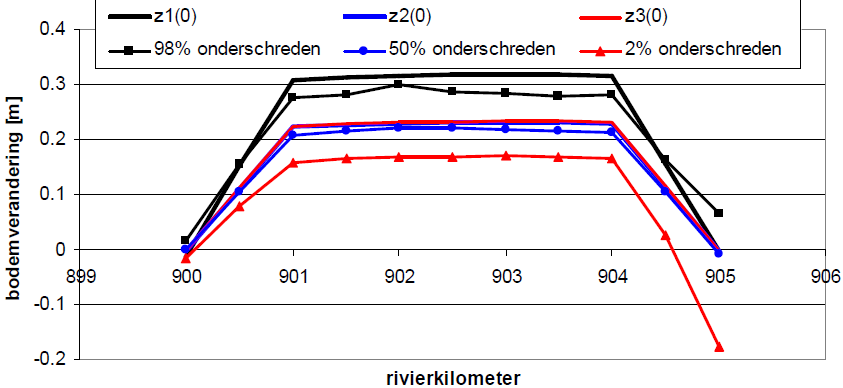
\includegraphics[width=\columnwidth]{figures/Fig9.png}
\caption{Estimated and simulated bed level changes at the secondary channel along the Waal.}
\label{App.Fig9}
\end{figure}

\subsection{Example 2: secondary channel along the Lek}

The second case also concerns a secondary channel; however, this time a secondary channel along the Lek between km 930 and km 935.
Also this secondary channel has been schematized as a local lateral extraction of flow from the overall river.
This extraction corresponds again to 3 \% of the total discharge for values up to 4000 m\textsuperscript{3}/s and increases linearly beyond to that 10 \% at 7000 m\textsuperscript{3}/s and higher discharges.
The effect on the main channel discharge is shown for a number of representative cross-sections in \autoref{App.Fig10}.

\begin{figure}
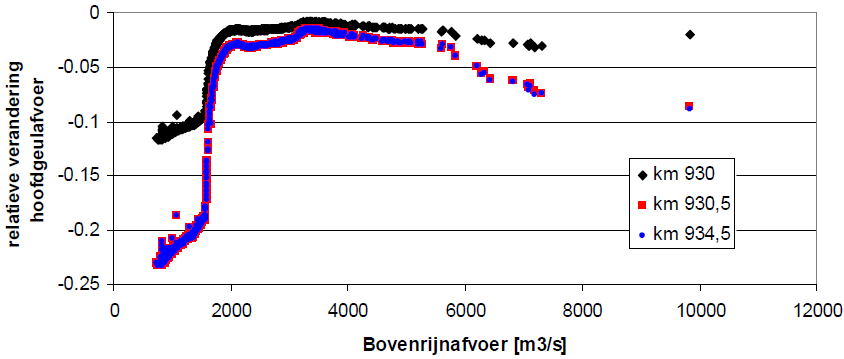
\includegraphics[width=\columnwidth]{figures/Fig10.png}
\caption{Influence of the secondary channel on the main channel discharge for the Lek}
\label{App.Fig10}
\end{figure}

\subsubsection*{Step 1) Characterize the intervention}

The secondary channel extracts 3 \% of the total discharge for Bovenrijn discharges up to 4000 m\textsuperscript{3}/s.
Above that value the withdrawal increases linearly up to 10 \% at 7000 m\textsuperscript{3}/s.
As in the first case there is no threshold discharge since the secondary channel is active for all discharges.
The reaches bankfull at a Bovenrijn discharge of 4000 m\textsuperscript{3}/s.

\subsubsection*{Step 2) Definition of the discharge blocks}

Because there is no threshold discharge the discharge $Q_1 = 1500$ m\textsuperscript{3}/s is used for the first (low flow) block.
For the second block (transitional discharges) applies that the secondary channel reaches bankfull at 4000 m\textsuperscript{3}/s, so $Q_2 = 4000$ m\textsuperscript{3}/s.
The discharge $Q_3$ of the third block (flood) is in agreement with \autoref{App.Tab7} equal to 6000 m\textsuperscript{3}/s.
These values can be used to compute the relative duration of each block as

\begin{itemize}
\item $Q_1=1500$ m\textsuperscript{3}/s implies $T_1 = 1-e^{\frac{800-1500}{1280}} = 0.42$
\item $Q_2=4000$ m\textsuperscript{3}/s implies $T_2 = e^{\frac{800-1500}{1280}} - e^{\frac{800-4000}{1280}} = 0.50$
\item $Q_3=6000$ m\textsuperscript{3}/s implies $T_3 = 1-T_1-T_2 = 0.08$
\end{itemize}

\subsubsection*{Step 3) Equilibrium bed level changes}

\begin{figure}
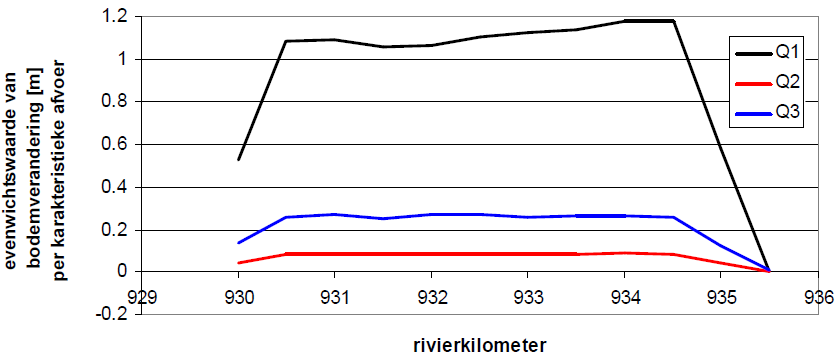
\includegraphics[width=\columnwidth]{figures/Fig11.png}
\caption{Equilibrium bed level changes in the main channel of the Lek at the site of the secondary channel.}
\label{App.Fig11}
\end{figure}

For each of the three characteristic discharges the equilibrium bed level changes were determined for each relevant cross-sectional profile based on the \sobek results as

\begin{equation}
\Delta z_{b,i,\text{eq}} = -h_o \frac{Q_{\text{main channel},n} - Q_{\text{main channel},o}}{Q_{\text{main channel},o}}
\end{equation}

\Note Usually the results of a 2D model are used for each individual computational point in the main channel.
However, for this application based on \sobek results the total main channel discharge and the average main channel depth were used which thus only verifies the impact along a single stream path.

The resulting equilibrium values are shown in \autoref{App.Fig11}.

\subsubsection*{Step 4) Time scales for relaxation}

The main channel width (normal width between groyne heads) at the site of the secondary channel is 140 m.
The bed celerity for low discharges is 0 m/yr; for high discharges this increases to 3120 m/yr.
Consequently, for each block we can compute

\begin{align}
\sigma_1 &= e^{-\frac{w_l}{2B_n}T_1} = e^{-\frac{0}{2 \cdot 140} 0.42} = 1.00 \\
\sigma_2 &= e^{-\frac{w_l}{2B_n}T_2} = e^{-\frac{3120}{2 \cdot 140} 0.50} = 0.004 \\
\sigma_3 &= e^{-\frac{w_l}{2B_n}T_3} = e^{-\frac{3120}{2 \cdot 140} 0.08} = 0.40
\end{align}

\subsubsection*{Step 5) Computation of the characteristic bed level changes}

Based on the equilibrium values determined in step 3 and the relaxation factors of step 4 the characteristic bed level changes can be computed.
For instance for cross-sectional profile km 930.5 we obtain $\Delta z_{b,1,\text{eq}} = 1.08$ m; $\Delta z_{b,2,\text{eq}} = 0.08$ m; $\Delta z_{b,3,\text{eq}} = 0.26$ m.
Substitution of these values into the appropriate equations gives for km 930.5

\begin{align}
z_{b,1}(0) &= \tfrac{1.08 \cdot (1-1.00) \cdot 0.004 \cdot 0.40 + 0.08 \cdot (1-0.004) \cdot 0.40 + 0.26 \cdot (1-0.40)}{1 - 1.00 \cdot 0.004 \cdot 0.40} = 0.20 \\
z_{b,2}(0) &= \tfrac{1.08 \cdot (1-1.00) + 0.08 \cdot (1-0.004) \cdot 0.40 \cdot 1.00 + 0.26 \cdot (1-0.40) \cdot 1.00}{1 - 1.00 \cdot 0.004 \cdot 0.40} = 0.20 \\
z_{b,3}(0) &= \tfrac{1.08 \cdot (1-1.00) \cdot 0.004 + 0.08 \cdot (1-0.004) + 0.26 \cdot (1-0.40) \cdot 1.00 \cdot 0.004}{1 - 1.00 \cdot 0.004 \cdot 0.40} = 0.08
\end{align}

\subsubsection*{Step 6) Visualizing the results}

\begin{figure}
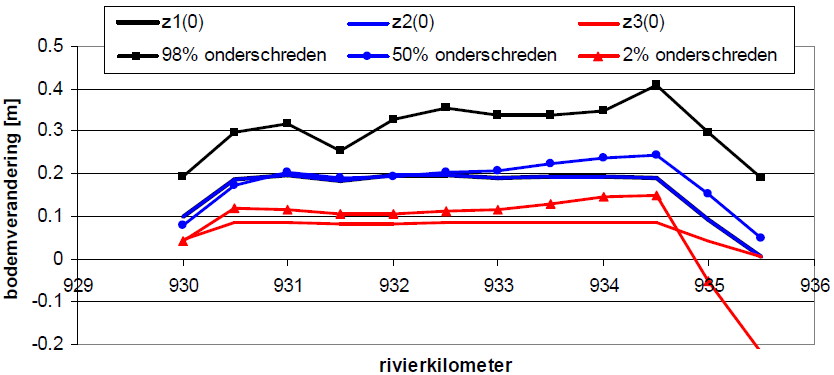
\includegraphics[width=\columnwidth]{figures/Fig12.png}
\caption{Estimated and simulated bed level changes at the secondary channel along the Lek.}
\label{App.Fig12}
\end{figure}

The alongstream profile of the characteristic bed level changes is shown together with the results obtained from \sobek in \autoref{App.Fig12}.
The $z_{b,1}(0)$ value (the characteristic maximum bed level change at the end of the flood period) corresponds in this case to the $z_{b,2}(0)$ value (the characteristic minimum bed level change at the end of the low flow period).
Both values correspond in this case well with the bed level change which is not exceeded during 50 \% of the time.
The $z_{b,3}(0)$ value corresponds in this particular case to the value not exceeded during 2 \% of the time.


\subsection{Example 3: an application to the Maas}

This example shows an analysis that was carried out using the original WAQMORF tool, but results of the latest \dfastmi program are consistent so it's still relevant.
The analysis was based on results obtained using the WAQUA model of "Over de Maas" of \citep{Svasek2007}.
The simulation results were provided by Ed Lemaire (DLB).

The test consisted of the following steps

\begin{enumerate}
\item The tool \dfastmi was used to determine the --- for the morphology --- representative discharges.
This step returned the discharges 1250 m\textsuperscript{3}/s, 1500 m\textsuperscript{3}/s and 2000 m\textsuperscript{3}/s at Borgharen.

\item WAQUA simulations were carried for both the reference situation and situation with the intervention implemented.
The water depths and flow velocities were exported using WAQVIEW to the export files supported by \dfastmi.

\item The export files were used as input for a second run of \dfastmi to estimate i) the mean annual bed level change, ii) the maximum bed level change (at the end of the flood season) and iii) the minimum bed level change (at the end of the low flow season)
\end{enumerate}

\begin{figure}
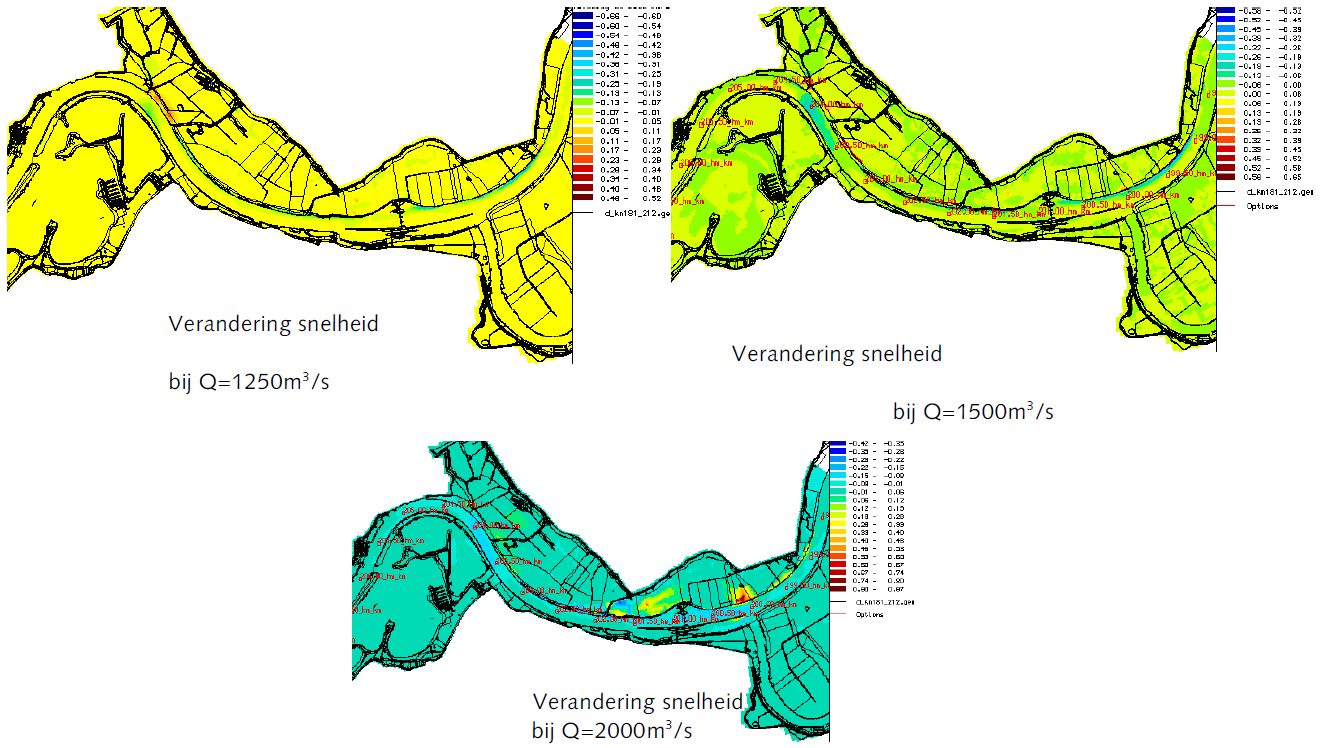
\includegraphics[width=\columnwidth]{figures/Fig13.png}
\caption{Overview of the velocity changes due to the intervention}
\label{App.Fig13}
\end{figure}

The biggest local bed level changes are located in the bend immediately downstream of the intervention.
The figures show the mean annual bed level changes in cm for three different critical velocities for the initiation of motion.
This parameter turns out to have little effect in this particular case.
The impact of the plan on river maintenance can be determined based on the available space in the navigation channel.

\begin{figure}
\center
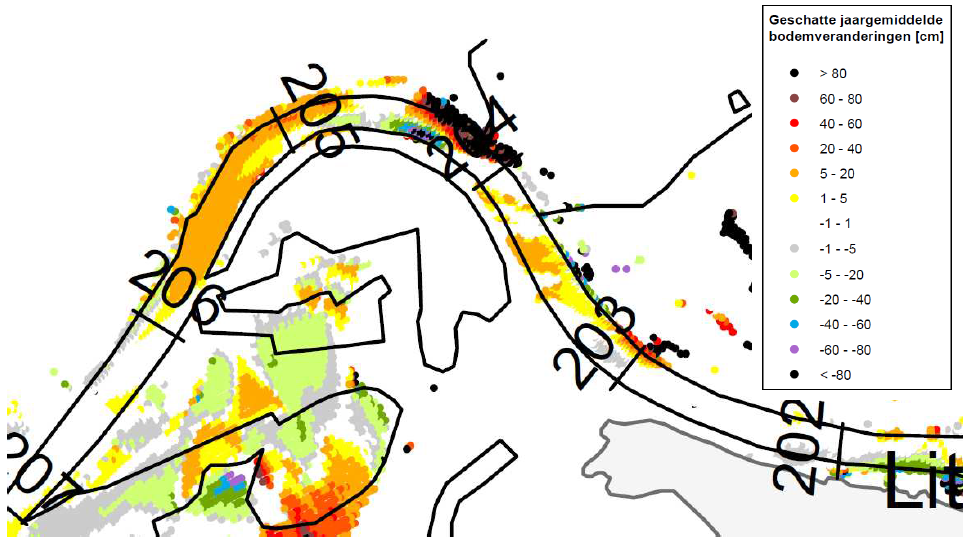
\includegraphics[width=12cm]{figures/Fig14a.png}
\caption{Estimated bed level changes (velocity threshold $u_{crit} = 0.01$ m/s).}
\label{App.Fig14a}
\end{figure}

\begin{figure}
\center
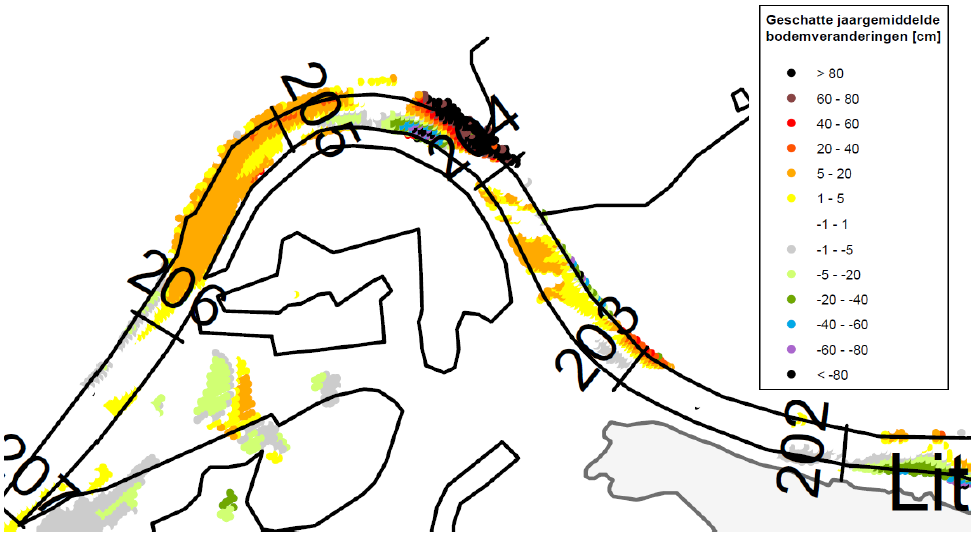
\includegraphics[width=12cm]{figures/Fig14b.png}
\caption{Estimated mean annual bed level changes (velocity threshold $u_{crit} = 0.10$ m/s).}
\label{App.Fig14b}
\end{figure}

\begin{figure}
\center
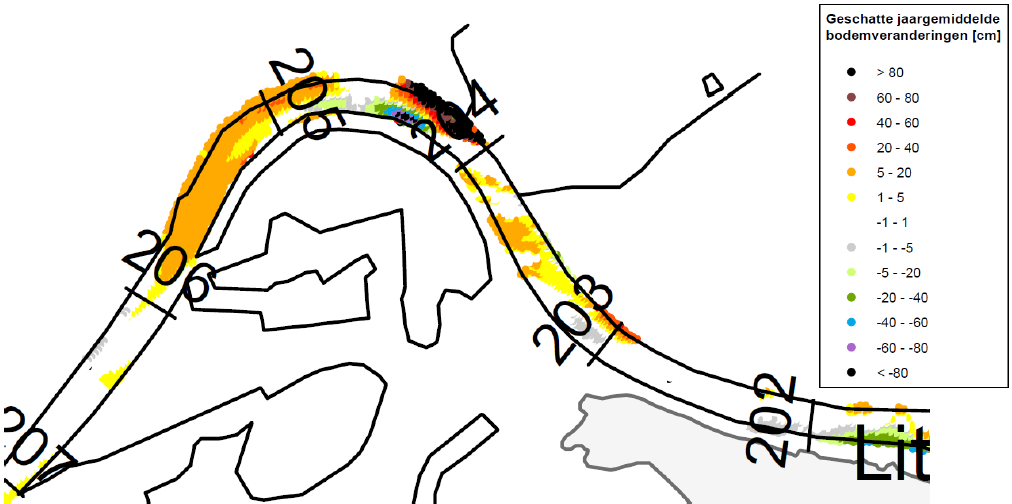
\includegraphics[width=12cm]{figures/Fig14c.png}
\caption{Estimated mean annual bed level changes (velocity threshold $u_{crit} = 0.30$ m/s).}
\label{App.Fig14c}
\end{figure}

\pagebreak[4]
\section{Example listing of the cli mode} \label{Sec:cli_dialog}

The following listing is an example of the interactive \keyw{cli} mode.

\begin{Verbatim}
This program implements the "WAQUA vuistregel" for the estimation of the local
morphological effects of a local intervention (i.e. an adjustment to the river). See
"RWS-WD memo WAQUA vuistregel 20-10-08" for details).

It is based on an estimation of the equilibrium bed level changes in the main
channel that would occur eventually when river maintenance would not be
adjusted.

The effect is expressed in [m] as:

    year-averaged bed level change without dredging
    maximum bed level change (after flood season) without dredging
    minimum bed level change (after low season) without dredging

By means of these estimates bottlenecks can be identified. The results are not
suitable for direct estimation of the impact on the maintenance of the
navigation channel!

The yearly sediment load of the river determines the period in which the
equilibrium can be reached.


This is version 3.0.0.

Confirm using "y" ...
\end{Verbatim}

You type \keyw{y}.

\begin{Verbatim}
The results are not valid for a combination of multiple interventions, or for a
single intervention extending over a distance more than 4 km!


In order to use D-FAST Morphological Impact you need to run reference and
scenario simulations on the same computational mesh.



The year discharge hydrograph is schematized using 3 blocks of constant
discharge:

    block 1 with discharge Q1 is the low water period
    block 2 with discharge Q2 is the transition period
    block 3 with discharge Q3 is the flood period


Are the simulation results already available?

Confirm using "y", or reply "n" ...
\end{Verbatim}

You type \keyw{y}.

\begin{Verbatim}
--------------------------------------------------------------------------------

The results of this program are three data files containing the characteristic
bed level changes. These files are:

    year-averaged change [m] without dredging in          "yearavg_dzb.out"
    maximum change [m] after flood without dredging in    "max_dzb.out"
    minimum change [m] after low flow without dredging in "min_dzb.out"

--------------------------------------------------------------------------------

Confirm using "y", or restart using "n" ...
\end{Verbatim}

You type \keyw{y}.

\begin{Verbatim}
On which branch is the intervention located?


    river branch                             nr

    Bovenrijn & Waal                         1

    Pannerdensch Kanaal & Nederrijn-Lek      2

    IJssel                                   3

    Merwedes                                 4

    Maas                                     5


The number of the river branch is ...
\end{Verbatim}

You type \keyw{1}.

\begin{Verbatim}
On which reach is the intervention located?


    river reach                             nr

    Bovenrijn                    km  859-867 1

    Boven-Waal                   km  868-886 2

    Midden-Waal                  km  887-915 3

    Beneden-Waal                 km  916-951 4


The number of the river reach is ...
\end{Verbatim}

You type \keyw{2}.

\begin{Verbatim}
--------------------------------------------------------------------------------

The intervention is located on reach Boven-Waal                   km  868-886

--------------------------------------------------------------------------------

Confirm using "y" or restart the location selection using "n" ...
\end{Verbatim}

You type \keyw{y}.

\begin{Verbatim}
The next three questions will be used to characterize the intervention. If an intervention
impacts the hydrodynamics in the main channel at multiple locations, answer the
questions for the part of the intervention that is expected to have the most impact
on the navigation channel.



Is the intervention flow-carrying for all discharges at Lobith above 1000 m3/s?

Confirm using "y", or reply "n" ...
\end{Verbatim}

You type \keyw{y}.

\begin{Verbatim}
Most of the flood plains become flow-carrying for discharges above 4000
m3/s. Is the intervention also bankfull for these discharges?

Confirm using "y", or reply "n" ...
\end{Verbatim}

You type \keyw{y}.

\begin{Verbatim}
Are the simulation results for Q1 = 3000.0  m3/s available?

Confirm using "y", or reply "n" ...
\end{Verbatim}

You type \keyw{y}.

\begin{Verbatim}
Are the simulation results for Q2 = 4000.0  m3/s available?

Confirm using "y", or reply "n" ...
\end{Verbatim}

You type \keyw{y}.

\begin{Verbatim}
Are the simulation results for Q3 = 6000.0  m3/s available?

Confirm using "y", or reply "n" ...
\end{Verbatim}

You type \keyw{y}.

\begin{Verbatim}
Below a certain velocity noo bed level changes occur.
The threshold value is set to  0.300000 m/s.

Is this an appropriate value for the reach Boven-Waal                   km  868-886?'

Confirm using "y", or reply "n" ...
\end{Verbatim}

You type \keyw{y}.

\begin{Verbatim}
Input of block 1 data files at Q=3000.0 m3/s

--------------------------------------------------------------------------------


The file name of flow velocity magnitudes without intervention is...
xyz_velocity-zeta.001.Q1.xyz
File "xyz_velocity-zeta.001.Q1.xyz" found!

The file name of water depths without intervention is...
xyz_waterdepth-zeta.001.Q1.xyz
File "xyz_waterdepth-zeta.001.Q1.xyz" found!

The file name of flow velocity magnitudes with intervention is...
xyz_velocity-zeta.002.Q1.xyz
File "xyz_velocity-zeta.002.Q1.xyz" found!

Reading the data files for block 1 ...


--------------------------------------------------------------------------------


Input of block 2 data files at Q=4000.0 m3/s

--------------------------------------------------------------------------------


The file name of flow velocity magnitudes without intervention is...
xyz_velocity-zeta.001.Q2.xyz
File "xyz_velocity-zeta.001.Q2.xyz" found!

The file name of water depths without intervention is...
xyz_waterdepth-zeta.001.Q2.xyz
File "xyz_waterdepth-zeta.001.Q2.xyz" found!

The file name of flow velocity magnitudes with intervention is...
xyz_velocity-zeta.002.Q2.xyz
File "xyz_velocity-zeta.002.Q2.xyz" found!

Reading the data files for block 2 ...


--------------------------------------------------------------------------------


Input of block 3 data files at Q=6000.0 m3/s

--------------------------------------------------------------------------------


The file name of flow velocity magnitudes without intervention is...
xyz_velocity-zeta.001.Q3.xyz
File "xyz_velocity-zeta.001.Q3.xyz" found!

The file name of water depths without intervention is...
xyz_waterdepth-zeta.001.Q3.xyz
File "xyz_waterdepth-zeta.001.Q3.xyz" found!

The file name of flow velocity magnitudes with intervention is...
xyz_velocity-zeta.002.Q3.xyz
File "xyz_velocity-zeta.002.Q3.xyz" found!

Reading the data files for block 3 ...


--------------------------------------------------------------------------------


Determining the characteristic bed level changes ...



If the bed level changes are removed on a yearly basis, the impacted river reach
is estimated at 1319 m from the upstream edge of the impacted reach.

Confirm using "y" to end the program ...
\end{Verbatim}

You type \keyw{y}.

\begin{Verbatim}
The program has ended !!!
\end{Verbatim}

\section{Old file formats}\label{app-v1:old-formats}

\subsection{Rivers configuration file}\label{app-v1:rivers}

The rivers configuration file follows the common ini-file format.
The file must contain a \keyw{[General]} block with a keyword \keyw{Version} to indicate the version number of the file.
The version number should be \keyw{1.0}.

Besides the \keyw{[General]} block version 1.0 files should only contain data blocks for the river branches (in Dutch: takken).
The names of those blocks will be used as branch names.
For instance, a block [My branch] will be processed as a branch called "My branch".
The order of the branches will correspond to the order of the blocks in the file.
The branch block defines the reaches (in Dutch: stukken) to be distinguished as well as the branch or reach specific parameter settings.
The \keyw{[General]} block may contain default values for the 
Further details follow below.

\begin{longtable}{l|l|p{8cm}}
\caption{Description of rivers configuration version 1} \\
Block & Keyword & Description \\ \hline
\endfirsthead
Block & Keyword & Description \\ \hline
      &         & \hfill\textsl{(continued from previous page)} \\ \hline
\endhead
      &         & \hfill\textsl{(continued on next page)} \\ \hline
\endfoot
\hline
\endlastfoot
\keyw{General} & \keyw{Version} & Version number. Must be \keyw{1.0}. \\
\keyw{General} & \keyw{Checksum} & Checksum of the rivers configuration file.
Used to verify whether the file wasn't accidentally modified. \\
BranchName<i> & \keyw{Reach<j>} & Name of reach <j> within branch <i> \\
BranchName<i> & \keyw{QLocation} & Location at which discharges for branch <i> are defined \\
\keyw{*} & \keyw{QStagnant} & Discharge \unitbrackets{m\textsuperscript{3}/s} below which main channel flow can be assumed stagnant \\
\keyw{*} & \keyw{QMin} & Minimum discharge \unitbrackets{m\textsuperscript{3}/s} at which intervention becomes active \\
\keyw{*} & \keyw{QFit} & Two discharges \unitbrackets{m\textsuperscript{3}/s} used for representing the exceedance curve \\
\keyw{*} & \keyw{QLevels} & Four characteristic discharges \unitbrackets{m\textsuperscript{3}/s} used by algorithm \\
\keyw{*} & \keyw{dQ} & Two discharge adjustments \unitbrackets{m\textsuperscript{3}/s} used by algorithm \\
\keyw{*} & \keyw{NWidth} & Normal width \unitbrackets{m} of main channel \\
\keyw{*} & \keyw{PRLow} & Low flow propagation rate \unitbrackets{km/yr} \\
\keyw{*} & \keyw{PRHigh} & High flow propagation rate \unitbrackets{km/yr} \\
\keyw{*} & \keyw{UCrit} & Critical (minimum) velocity \unitbrackets{m/s} for sediment transport
\end{longtable}

The second value of \keyw{QLevels} corresponds to the typical bankfull discharge.
All keywords listed for block \keyw{*} may occur either in the \keyw{[General]} block or in one of the branch specific blocks where they may optionally be concatenated with the reach number <j>.
Those keywords may thus occur in three flavours:

\begin{enumerate}
\item Plain keyword in block \keyw{[General]}: global default value valid for all branches
\item Plain keyword in branch specific block: default value for that branch (overrules any global default)
\item Keyword followed by reach number <j> in branch specific block: value valid for that reach on that branch.
\end{enumerate}

\subsubsection*{Example}

The following excerpt of the default \keyw{Dutch\_rivers.ini} configuration file shows the \keyw{[General]} as well as the first part of the \keyw{[Bovenrijn \& Waal]} block for the first branch.
It includes a global value of 0.3 for \keyw{UCrit} and 100 for \keyw{QMin}.
The other parameters are specified at branch level and mostly uniform for the whole branch.
Only \keyw{NWidth} and \keyw{PRLow} vary depending on the reach selected.

\begin{Verbatim}
    [General]
        Version    = 1.0

        UCrit      = 0.3
        QMin       = 1000

    [Bovenrijn & Waal]
        QLocation  = Lobith
        QStagnant  = 800
        QFit       = 800  1280
        QLevels    = 3000  4000  6000  10000
        dQ         = 1000  1000
        PRHigh     = 3.65
        
        Reach1     = Bovenrijn                    km  859-867
        NWidth1    = 340
        PRLow1     = 0.89
        
        Reach2     = Boven-Waal                   km  868-886
        NWidth2    = 260
        PRLow2     = 0.81

        ... continued ...
\end{Verbatim}

\subsection{Analysis configuration file}\label{app-v1:config}

The analysis configuration file follows the common ini-file format.
The file must contain a \keyw{[General]} block with a keyword \keyw{Version} to indicate the version number of the file.
The version number should be \keyw{1.0}.

Version 1.0 files must contain in the \keyw{[General]} block also the keywords \keyw{Branch} and \keyw{Reach} to identify the branch (in Dutch: tak) and reach (in Dutch: stuk) in which the intervention is located.
The specified names may be shortened, but they should uniquely identify the branch and reach amongst the names of the other branches and reaches.
Optionally, the same block may also contain \keyw{Qmin}, \keyw{QBankfull} and \keyw{UCrit} values representative for this particular intervention if they differ from those typical for the selected reach.
These items are sufficient for a basic analysis.
For a full spatial analysis the user needs to specify the names of the D-Flow FM map-files containing the results of the simulations without intervention (reference) and with intervention for the selected discharges Q1, Q2, and Q3.

\begin{tabular}{l|l|p{8cm}}
Block & Keyword & Description \\ \hline
\keyw{General} & \keyw{Version} & Version number. Must be \keyw{1.0}. \\
\keyw{General} & \keyw{Mode} & \keyw{WAQUA export} or \keyw{D-Flow FM map} (the latter is the default) \\
\keyw{General} & \keyw{Branch} & Name of the selected branch \\
\keyw{General} & \keyw{Reach} & Name of the selected reach \\
\keyw{General} & \keyw{QMin} & Minimum discharge \unitbrackets{m\textsuperscript{3}/s} at which intervention becomes active \\
\keyw{General} & \keyw{QBankfull} & Discharge \unitbrackets{m\textsuperscript{3}/s} at which intervention reaches bankfull \\
\keyw{General} & \keyw{UCrit} & Critical (minimum) velocity \unitbrackets{m/s} for sediment transport \\
\keyw{Q1} & \keyw{Discharge} & Discharge \unitbrackets{m\textsuperscript{3}/s} of the low flow simulation \\
\keyw{Q1} & \keyw{Reference} & Name of D-Flow FM map-file to be used for reference condition at Q1 \\
\keyw{Q1} & \keyw{WithMeasure} & Name of D-Flow FM map-file that includes the intervention at Q1 \\
\keyw{Q2} & \keyw{Discharge} & Discharge \unitbrackets{m\textsuperscript{3}/s} of the transitional regime \\
\keyw{Q2} & \keyw{Reference} & Name of D-Flow FM map-file to be used for reference condition at Q2 \\
\keyw{Q2} & \keyw{WithMeasure} & Name of D-Flow FM map-file that includes the intervention at Q2 \\
\keyw{Q3} & \keyw{Discharge} & Discharge \unitbrackets{m\textsuperscript{3}/s} of the high flow simulation \\
\keyw{Q3} & \keyw{Reference} & Name of D-Flow FM map-file to be used for reference condition at Q3 \\
\keyw{Q3} & \keyw{WithMeasure} & Name of D-Flow FM map-file that includes the intervention at Q3 \\
\end{tabular}

The file names may be specified using relative or absolute paths.
The \keyw{Reference} and \keyw{WithMeasure} keywords are *not* used when the \keyw{Mode} equals \keyw{WAQUA export}; in that case the file name are standardized as \keyw{xyz\_<quantity>-zeta.00<1/2>.Q<i>}.

\subsubsection*{Example}

This example shows a complete analysis configuration file for an intervention in the first branch/reach of the default \keyw{Dutch\_rivers.cfg} configuration.
It reports the default settings.
Only the \keyw{Version}, \keyw{Branch}, \keyw{Reach}, \keyw{Reference} and \keyw{WithMeasure} keywords are required for the full analysis.

\begin{Verbatim}
    [General]
      Version     = 1.0
      Mode        = D-Flow FM map
      Branch      = Bovenrijn & Waal
      Reach       = Bovenrijn                    km  859-867
      Qmin        = 1000.0
      Qbankfull   = 4000.0
      Ucrit       = 0.3
    
    [Q1]
      Discharge   = 1000.0
      Reference   = Measure42/Q1/Reference/DFM_OUTPUT_Q1/Q1_map.nc
      WithMeasure = Measure42/Q1/Updated/DFM_OUTPUT_Q1/Q1_map.nc
    
    [Q2]
      Discharge   = 4000.0
      Reference   = Measure42/Q2/Reference/DFM_OUTPUT_Q2/Q2_map.nc
      WithMeasure = Measure42/Q2/Updated/DFM_OUTPUT_Q2/Q2_map.nc
    
    [Q3]
      Discharge   = 6000.0
      Reference   = Measure42/Q3/Reference/DFM_OUTPUT_Q3/Q3_map.nc
      WithMeasure = Measure42/Q3/Updated/DFM_OUTPUT_Q3/Q3_map.nc
\end{Verbatim}


\section{Simulation result files}

The latest updates of \dfastmi only work using input data in UGRID netCDF files as obtained from \dflowfm.
Results obtained from Delft3D-FLOW and WAQUA can be converted to this format by means of \keyw{sim2ugrid}, a MATLAB-based conversion tool included in the QUICKPLOT distribution.

In backward compatibility mode, \dfmi can also read the same WAQUA files as used by WAQMORF.
The WAQUA simulation engine writes the simulation results in a proprietary SDS file format.
The content of these result files can't be accessed directly from Python, so they need to be exported to a more accessible file format.
The previous WAQMORF program also required that the user extracted the cell centred velocity magnitude and water depth values from the the WAQUA SDS-output files write them to simple ASCII files with 6 columns specifying the x-coordinates, y-coordinates, the value of the quantity (labeled as z-coordinate), m-index, n-index, and cell number.
Only the "z" values and the m- and n-indices are used by the program.
The names of those files has been hardcoded, they should read \keyw{xyz\_<quantity>-zeta.00<1/2>.Q<i>} with the quantity name equal to 'velocity' or 'waterdepth', a 1 for the reference simulation and a 2 for the simulation with the intervention implemented, and i the number of the discharge level.
\dfastmi supports these same files; an example of such file are given below.

\subsubsection*{Example}

\begin{Verbatim}
x,y,z,m,n,id
     197940.645,     431152.719,         0.0000,     2,     1,        11
     197874.004,     431430.516,         0.0000,     3,     1,        12
     197801.719,     431717.008,         0.0000,     4,     1,        13
     197727.047,     431985.375,         0.0000,     5,     1,        14
     197658.695,     432196.953,         0.0000,     6,     1,        15
     197610.234,     432323.859,         0.0000,     7,     1,        16
     197581.203,     432391.383,         0.0000,     8,     1,        17
     197559.625,     432439.234,         0.0000,     9,     1,        18
     197542.594,     432476.234,         0.0000,    10,     1,        19
     197528.668,     432506.070,         0.0000,    11,     1,        20
     197515.137,     432535.016,         0.0000,    12,     1,        21
     197505.176,     432556.258,         0.6156,    13,     1,        22
     197496.215,     432575.305,         0.8334,    14,     1,        23
     197485.773,     432597.516,         0.9794,    15,     1,        24
     197475.344,     432619.711,         1.0762,    16,     1,        25
     197465.578,     432640.484,         1.1305,    17,     1,        26
     197456.320,     432660.203,         1.1674,    18,     1,        27
     197447.242,     432679.563,         1.2085,    19,     1,        28
     197438.004,     432699.258,         1.2506,    20,     1,        29
     197428.273,     432720.000,         1.2913,    21,     1,        30
     197417.879,     432742.133,         1.3212,    22,     1,        31 

... continued ...
\end{Verbatim}


\subsection{Spatial output file}

The WAQMORF program wrote the spatial output in SIMONA BOX-file format which could be visualize when combined with the curvilinear grid of the original simulation.
\dfastmi still generates such files when run based on WAQUA results.
